\begin{frame}
\frametitle{Example 2: Sudoku}
\begin{itemize}
\item Global Constraints
\begin{itemize}
\item Powerful modelling abstractions
\item Non-trivial propagation
\item Different consistency levels
\end{itemize}
\item Example: Sudoku puzzle
\end{itemize}
\end{frame}

\section{Problem}

\begin{frame}<presentation>
\frametitle{Problem Definition}
\begin{block}{Sudoku}
Fill in numbers from 1 to 9 so that each row, column and $3x3$ block contain each number exactly once
\end{block}
\begin{center}
\begin{tabular}{cc}
\only<1->{\includegraphics[width=3.5cm]{../sudoku/../sudoku/DC/frame1}}
&
\only<2>{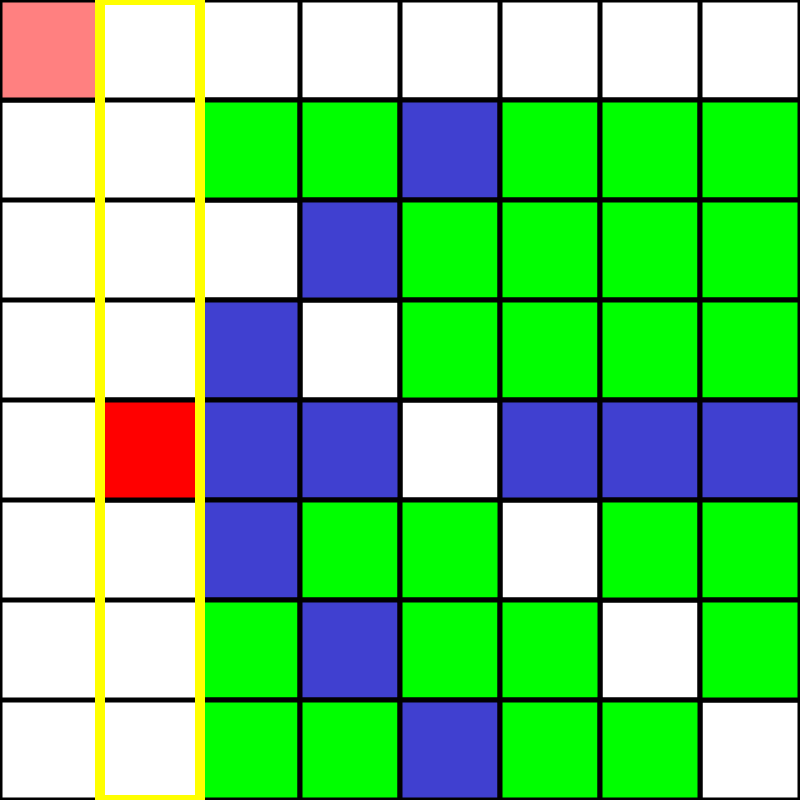
\includegraphics[width=3.5cm]{../sudoku/../sudoku/DC/frame31}}
\end{tabular}
\end{center}
\end{frame}

\begin{figure}[ht]
\caption{\label{sudoku:example}Example Problem and Solution}
\begin{center}
\begin{tabular}{cc}
\only<1->{\includegraphics[width=5cm]{../sudoku/../sudoku/DC/frame1}}
&
\only<2>{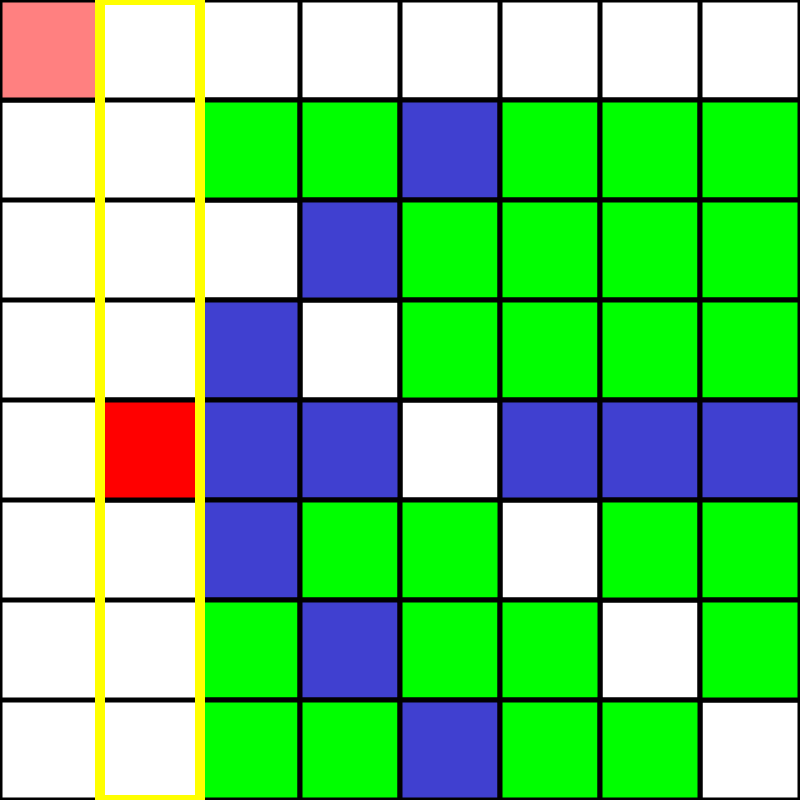
\includegraphics[width=5cm]{../sudoku/../sudoku/DC/frame31}}
\end{tabular}
\end{center}
\end{figure}

\begin{frame}
\frametitle{Model}
\begin{itemize}
\item A variable for each cell, ranging from 1 to 9
\item A 9x9 matrix of variables describing the problem
\item Preassigned integers for the given hints
\item \pred{alldifferent} constraints for each row, column and 3x3 block
\end{itemize}
\end{frame}

% \begin{frame}
% \frametitle{Reminder: \pred{alldifferent}}
% \begin{itemize}
% \item Argument: list of variables
% \item Meaning: variables are pairwise different
% \item Reasoning: Forward Checking (FC)
% \begin{itemize}
% \item When variable is assigned to value, remove the value from all other variables
% \item If a variable has only one possible value, then it is assigned
% \item If a variable has no possible values, then the constraint fails
% \item Constraint is checked whenever one of its variables is assigned
% \item Equivalent to decomposition into binary disequality constraints
% \end{itemize}
% \end{itemize}
% \end{frame}

\begin{frame}
\frametitle{Sudoku Models}
\begin{itemize}
\item ECLiPSe \hyperlink{sudoku:eclipse}{\beamergotobutton{Show}}
\item MiniZinc \hyperlink{sudoku:minizinc}{\beamergotobutton{Show}}
\item NumberJack \hyperlink{sudoku:numberjack}{\beamergotobutton{Show}}
\item CPMpy \hyperlink{sudoku:cpmpy}{\beamergotobutton{Show}}
\item Choco-solver \hyperlink{sudoku:choco}{\beamergotobutton{Show}}
\end{itemize}
\end{frame}

\begin{frame}[fragile]
\frametitle{ECLiPSe Sudoku Model {\small(from \url{https://eclipseclp.org/})}}
\label{sudoku:eclipse}
\tiny
\begin{verbatim}
:- lib(ic).
:- import alldifferent/1 from ic_global.

top :-
    problem(Board),
    print_board(Board),
    sudoku(Board),
    labeling(Board),
    print_board(Board).

sudoku(Board) :-
    dim(Board, [N,N]),
    Board :: 1..N,
    ( for(I,1,N), param(Board) do
        alldifferent(Board[I,*]),
        alldifferent(Board[*,I])
    ),
    NN is integer(sqrt(N)),
    ( multifor([I,J],1,N,NN), param(Board,NN) do
        alldifferent(concat(Board[I..I+NN-1, J..J+NN-1]))
    ).

print_board(Board) :-
    dim(Board, [N,N]),
    ( for(I,1,N), param(Board,N) do
        ( for(J,1,N), param(Board,I) do
        X is Board[I,J],
        ( var(X) -> write("  _") ; printf(" %2d", [X]) )
        ), nl
    ), nl.
\end{verbatim}
\end{frame}

\begin{frame}[fragile]
\frametitle{ECLiPSe Data Definition}
\tiny
\begin{verbatim}
problem([](
    [](4, _, 8, _, _, _, _, _, _),
    [](_, _, _, 1, 7, _, _, _, _),
    [](_, _, _, _, 8, _, _, 3, 2),
    [](_, _, 6, _, _, 8, 2, 5, _),
    [](_, 9, _, _, _, _, _, 8, _),
    [](_, 3, 7, 6, _, _, 9, _, _),
    [](2, 7, _, _, 5, _, _, _, _),
    [](_, _, _, _, 1, 4, _, _, _),
    [](_, _, _, _, _, _, 6, _, 4))).
\end{verbatim}
\hyperlink{sudoku:continue}{\beamergotobutton{Continue}}
\end{frame}



\begin{frame}[fragile]
\frametitle{MiniZinc Sudoku Model}
\label{sudoku:minizinc}
\tiny
\begin{semiverbatim}
int: s;
int: n=s*s;
array[1..n,1..n] of var 1..n: puzzle;

include "sudoku.dzn";

predicate alldifferent(array[int] of var int: x) =
  forall(i,j in index_set(x) where i < j)
    (x[i] != x[j]); 
    
constraint forall(i in 1..n)
    (alldifferent([puzzle[i,j]| j in 1..n]));
constraint forall(j in 1..n)
    (alldifferent([ puzzle[i,j]| i in 1..n]));
constraint forall(i,j in 1..s)
    (alldifferent([puzzle[s*(i-1)+p, s*(j-1)+q]|
                  p,q in 1..s]));
solve satisfy;
\end{semiverbatim}
\end{frame}

\begin{frame}[fragile]
\frametitle{MiniZinc Output}
\tiny
\begin{verbatim}
output [ "sudoku:\\n" ] ++
  [ show(puzzle[i,j]) ++
    if j = n then
       if i mod s = 0 /\ i < n then "\n\n"
       else "\n"
       endif
     else
       if j mod s = 0 then "  "
       else " "
       endif
     endif
    | i,j in 1..n ];
\end{verbatim}
\end{frame}

\begin{frame}[fragile]
\frametitle{MiniZinc Data File {\tiny(sudoku.dzn)}}
\tiny
\begin{semiverbatim}
s=3;
puzzle=[|
    4, _, 8, _, _, _, _, _, _|
    _, _, _, 1, 7, _, _, _, _|
    _, _, _, _, 8, _, _, 3, 2|
    _, _, 6, _, _, 8, 2, 5, _|
    _, 9, _, _, _, _, _, 8, _|
    _, 3, 7, 6, _, _, 9, _, _|
    2, 7, _, _, 5, _, _, _, _|
    _, _, _, _, 1, 4, _, _, _|
    _, _, _, _, _, _, 6, _, 4|
|];
\end{semiverbatim}
\hyperlink{sudoku:continue}{\beamergotobutton{Continue}}
\end{frame}

\begin{frame}[fragile]
\frametitle{NumberJack Sudoku Model}
\label{sudoku:numberjack}
\tiny
\begin{verbatim}
from Numberjack import *

def get_model(N, clues):
    grid = Matrix(N*N, N*N, 1, N*N)

    sudoku = Model([AllDiff(row) for row in grid.row],
                   [AllDiff(col) for col in grid.col],
                   [AllDiff(grid[x:x + N, y:y + N]) for x in range(0, N*N, N) 
                                                    for y in range(0, N * N, N)],
                   [(x == int(v)) for x, v in 
                       zip(grid.flat, "".join(open(clues)).split()) if v != '*']
                   )
    return grid, sudoku

def solve(param):
    N = param['N']
    clues = param['file']

    grid, sudoku = get_model(N, clues)

    solver = sudoku.load(param['solver'])
    solver.setVerbosity(param['verbose'])
    solver.setTimeLimit(param['tcutoff'])

    solver.solve()
\end{verbatim}
\end{frame}

\begin{frame}[fragile]
\frametitle{NumberJack Data File}
\tiny
\begin{verbatim}
4 * 8 * * * * * *
* * * 1 7 * * * *
* * * * 8 * * 3 2
* * 6 * * 8 2 5 *
* 9 * * * * * 8 *
* 3 7 6 * * 9 * *
2 7 * * 5 * * * *
* * * * 1 4 * * *
* * * * * * 6 * 4
\end{verbatim}
\hyperlink{sudoku:continue}{\beamergotobutton{Continue}}
\end{frame}



\begin{frame}[fragile]
\frametitle{CPMpy Sudoku Model{\small(from \url{https://github.com/CPMpy/})}}
\label{sudoku:cpmpy}
\tiny
\begin{verbatim}
import numpy as np
from cpmpy import *

# Variables
puzzle = intvar(1,9, shape=given.shape, name="puzzle")

model = Model(
    # Constraints on values (cells that are not empty)
    puzzle[given!=e] == given[given!=e], # numpy's indexing, vectorized equality
    # Constraints on rows and columns
    [AllDifferent(row) for row in puzzle],
    [AllDifferent(col) for col in puzzle.T], # numpy's Transpose
)

# Constraints on blocks
for i in range(0,9, 3):
    for j in range(0,9, 3):
        model += AllDifferent(puzzle[i:i+3, j:j+3]) # python's indexing

model.solve()
\end{verbatim}
\end{frame}

\begin{frame}[fragile]
\frametitle{CPMpy Data Definition}
\tiny
\begin{verbatim}
e = 0 # value for empty cells
given = np.array([
    [4, e, 8, e, e, e, e, e, e],
    [e, e, e, 1, 7, e, e, e, e],
    [e, e, e, e, 8, e, e, 3, 2],
    [e, e, 6, e, e, 8, 2, 5, e],
    [e, 9, e, e, e, e, e, 8, e],
    [e, 3, 7, 6, e, e, 9, e, e],
    [2, 7, e, e, 5, e, e, e, e],
    [e, e, e, e, 1, 4, e, e, e],
    [e, e, e, e, e, e, 6, e, 4]
])
\end{verbatim}
\hyperlink{sudoku:continue}{\beamergotobutton{Continue}}
\end{frame}

\begin{frame}[fragile]
\frametitle{Choco-solver Sudoku Model}
\label{sudoku:choco}
\tiny
\begin{verbatim}
    Model model = new Model("Sudoku");
    int blockSize = 3;
    int m = blockSize*blockSize;

    IntVar[][] vars = new IntVar[m][m];
    for(int i=0;i<m;i++){
        for(int j=0;j<m;j++){
            vars[i][j] =  model.intVar("X"+i+""+j, 1, m);
            if (data[i][j]>0) {
                model.arithm(vars[i][j],"=",data[i][j]).post();
            }
        }
    }
    for(int i=0;i<m;i++){
        model.allDifferent(row(i,m,vars)).post();
        model.allDifferent(column(i,m,vars)).post();
    }
    for(int i=0;i<m;i+=blockSize){
        for(int j=0;j<m;j+=blockSize){
            model.allDifferent(block(i,j,blockSize,vars)).post();
        }
    }
    Solver solver = model.getSolver();
    solver.solve();
\end{verbatim}
\end{frame}

\begin{frame}[fragile]
\frametitle{Choco-solver Data}
\tiny
\begin{verbatim}
int[][] data = new int[m][m]{
    {4, 0, 8, 0, 0, 0, 0, 0, 0},
    {0, 0, 0, 1, 7, 0, 0, 0, 0},
    {0, 0, 0, 0, 8, 0, 0, 3, 2},
    {0, 0, 6, 0, 0, 8, 2, 5, 0},
    {0, 9, 0, 0, 0, 0, 0, 8, 0},
    {0, 3, 7, 6, 0, 0, 9, 0, 0},
    {2, 7, 0, 0, 5, 0, 0, 0, 0},
    {0, 0, 0, 0, 1, 4, 0, 0, 0},
    {0, 0, 0, 0, 0, 0, 6, 0, 4}
};
\end{verbatim}
\end{frame}

\begin{frame}[fragile]
\frametitle{Choco-solver Utilities}
\tiny
\begin{verbatim}
IntVar[] row(int row, int size, IntVar[][] array){
    return array[row];
}

IntVar[] column(int col,int size,IntVar[][] array){
    IntVar[] column = new IntVar[size];
    for(int i=0; i<size; i++){
        column[i] = array[i][col];
    }
    return column;
}

IntVar[] block(int x,int y,int blockSize,IntVar[][] array){
    IntVar[] block = new IntVar[blockSize*blockSize];
    int k=0;
    for(int i=0;i<blockSize;i++){
        for(int j=0;j<blockSize;j++){
            block[k++] = array[x+i][y+j];
        }
    }
    return block;
}
\end{verbatim}
\hyperlink{sudoku:continue}{\beamergotobutton{Continue}}
\end{frame}

% \begin{frame}
  % \frametitle{Running sudoku\_decompose.mzn}
  % 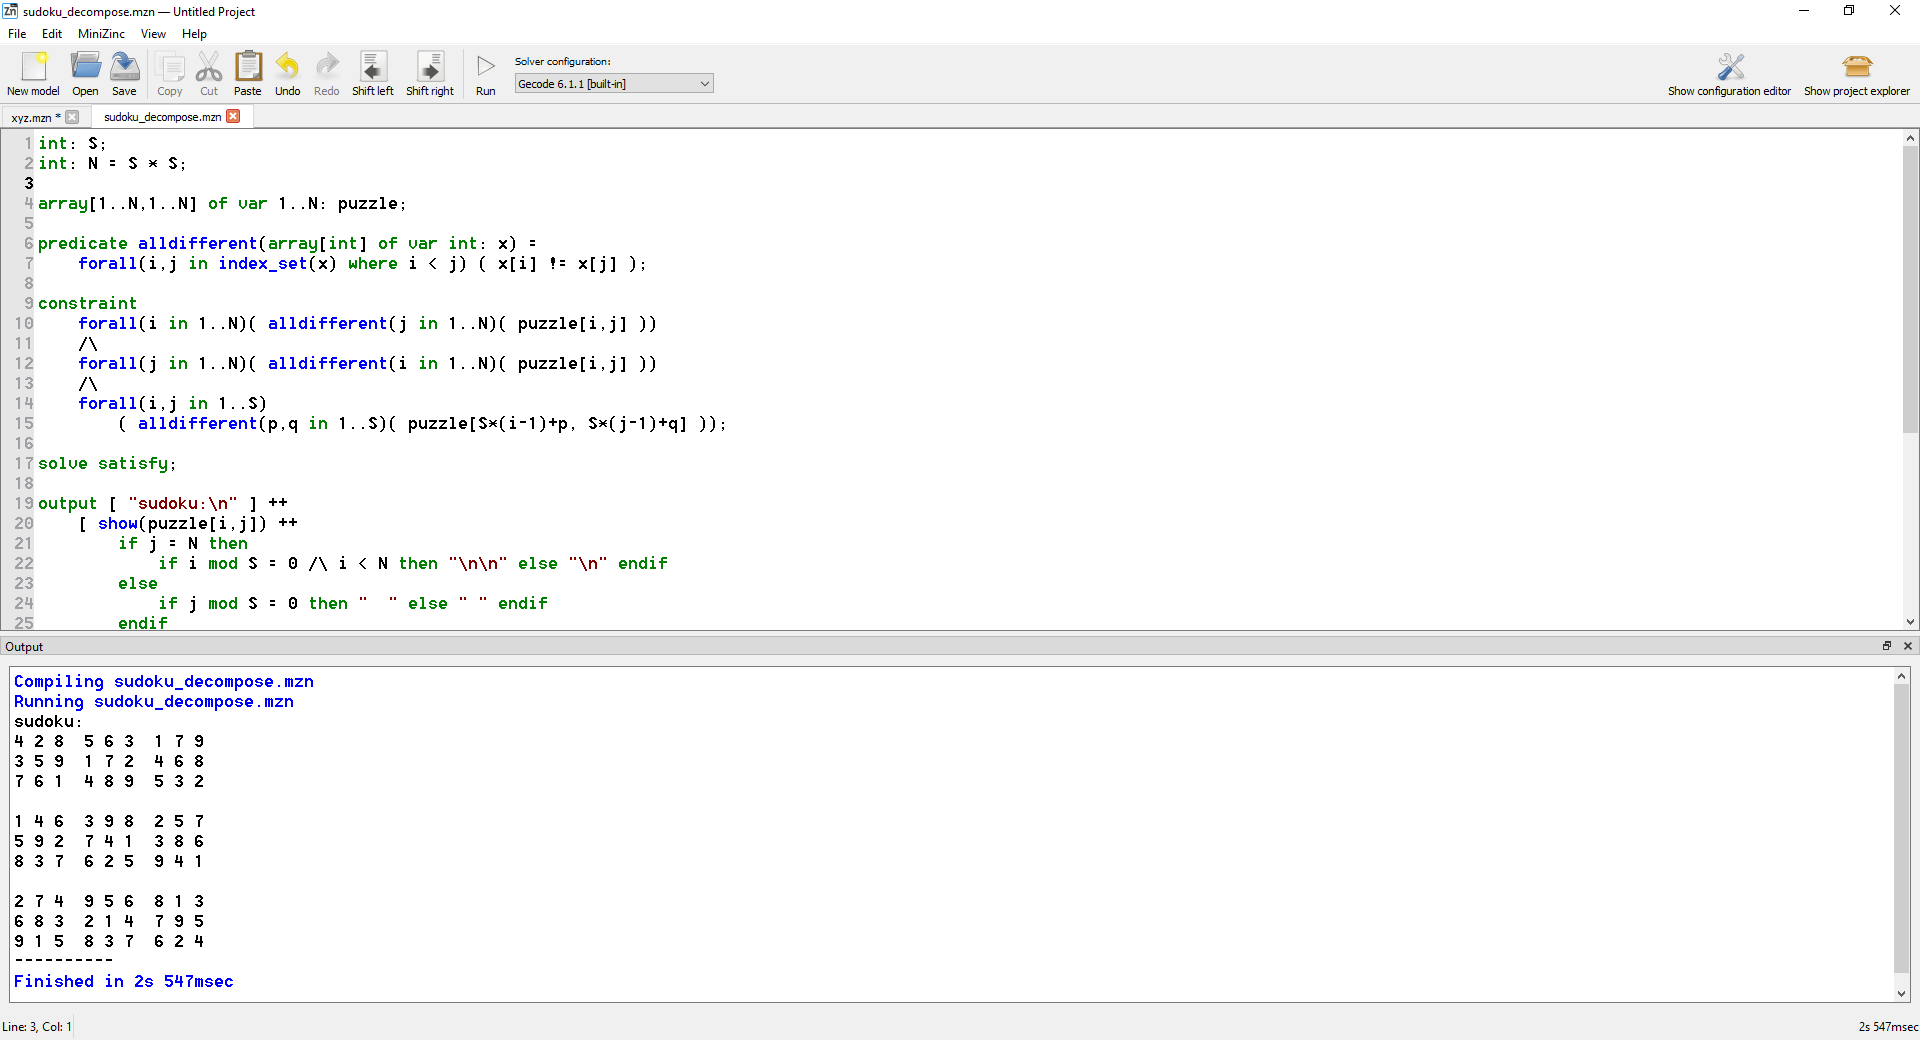
\includegraphics[width=10cm]{../sudoku/images/idesudoku}
  % \end{frame}

\begin{frame}
\frametitle{Domain Visualizer}
\label{sudoku:continue}
\only<presentation>{
\begin{textblock}{5.5}(10,-2)
\includegraphics[width=3.5cm]{../sudoku/FC/frame1}
\end{textblock}
}
\begin{itemize}
\item Problem shown as matrix
\item Each cell corresponds to a variable
\item Instantiated: Shows integer value (large)
\item Uninstantiated: Shows values in domain
\end{itemize}
\end{frame}

\clearpage
\section{Initial Propagation (Forward Checking)}

\begin{frame}<presentation>
\frametitle{Initial State (Forward Checking)}
\includegraphics[width=6cm]{../sudoku/FC/frame1}
\end{frame}

\begin{figure}[ht]
\caption{\label{sudoku:initialstatefc}Initial State (Forward Checking)}
\begin{center}
\includegraphics[width=6cm]{../sudoku/FC/frame1}
\end{center}
\end{figure}


\begin{frame}<presentation>
\frametitle{Propagation Steps (Forward Checking)}
\only<beamer>{
\only<1>{\includegraphics[width=6cm]{../sudoku/FC/frame1}}
\only<2>{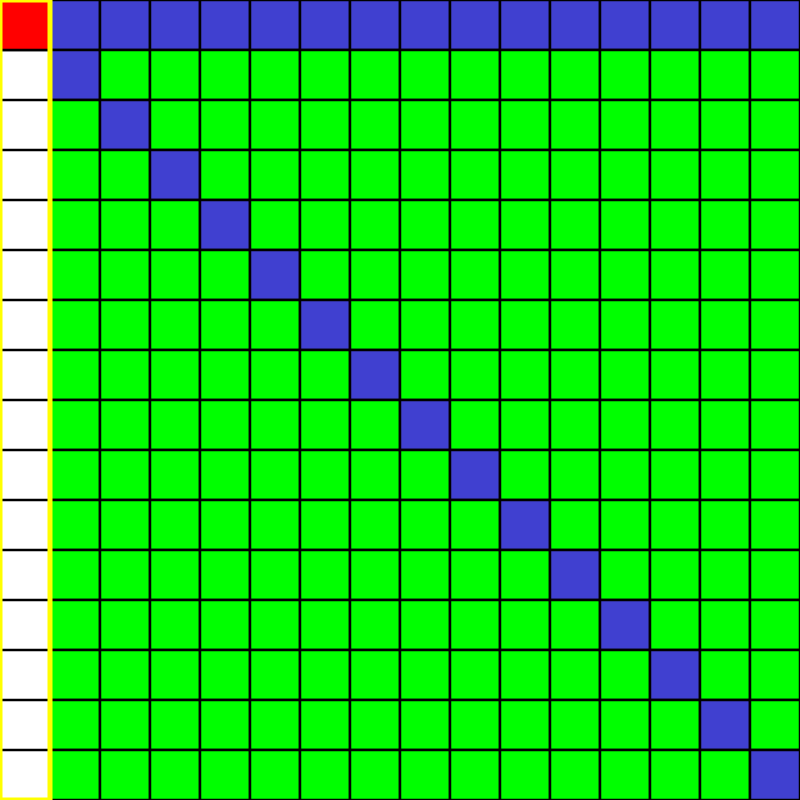
\includegraphics[width=6cm]{../sudoku/FC/frame2}}
\only<3>{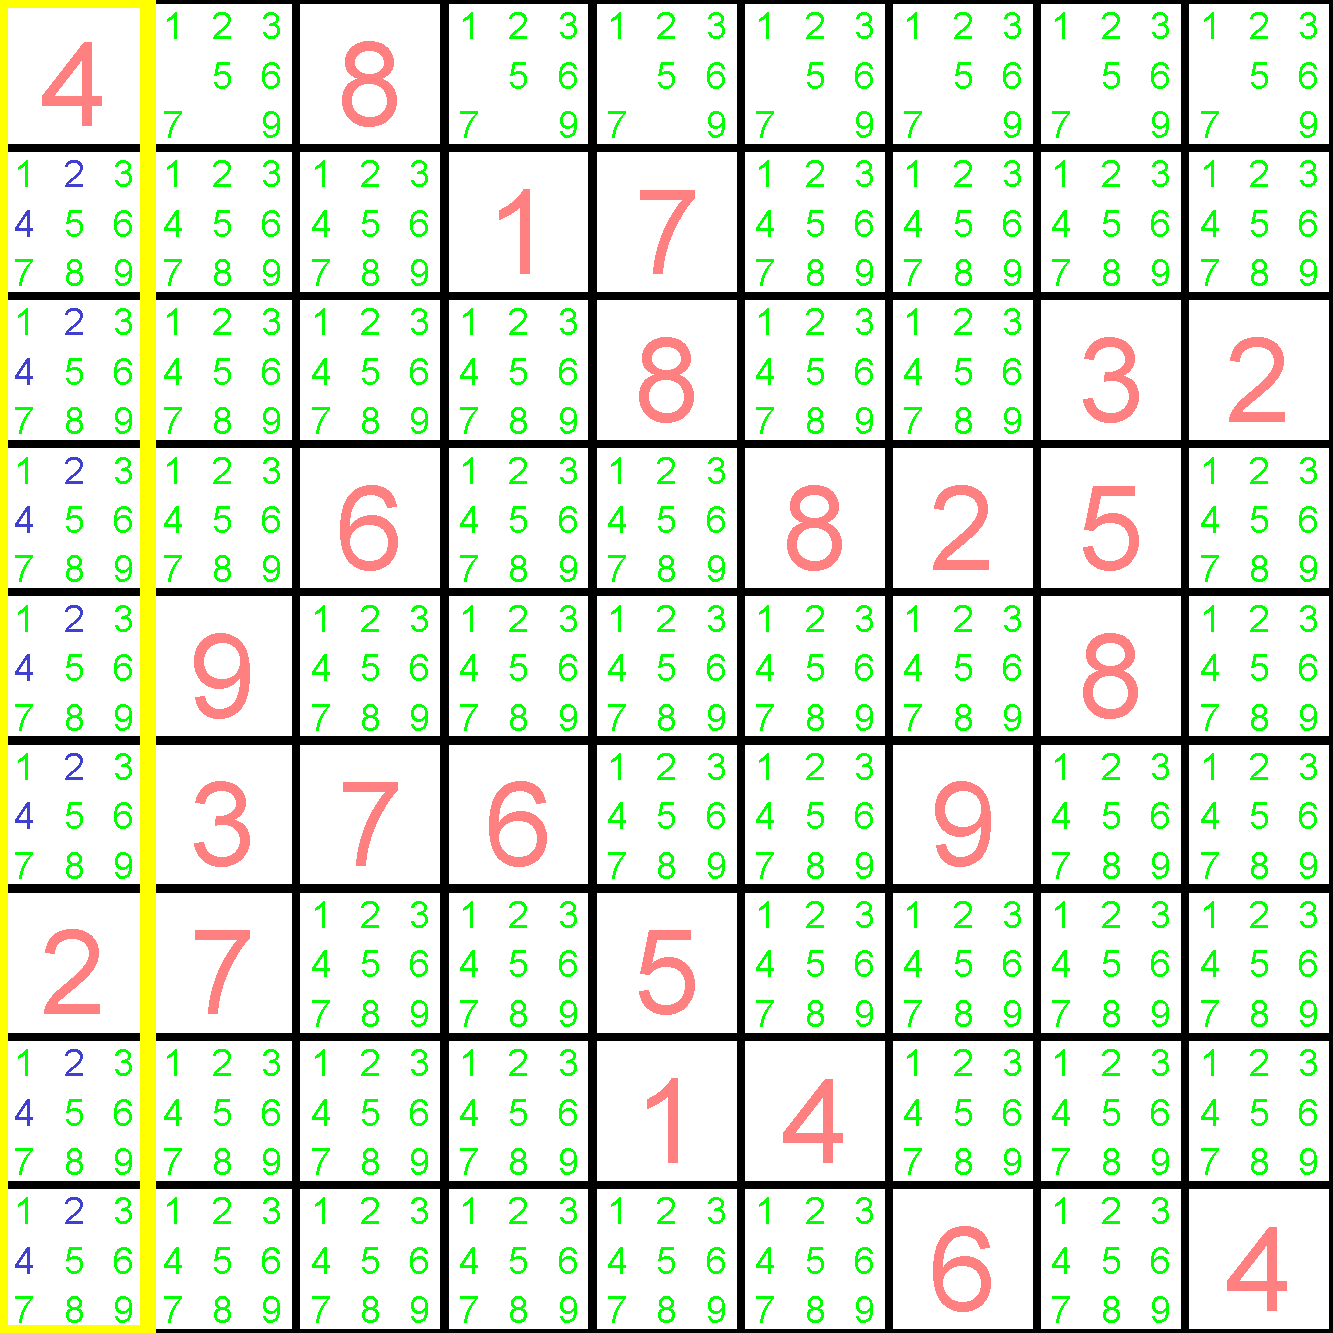
\includegraphics[width=6cm]{../sudoku/FC/frame3}}
\only<4>{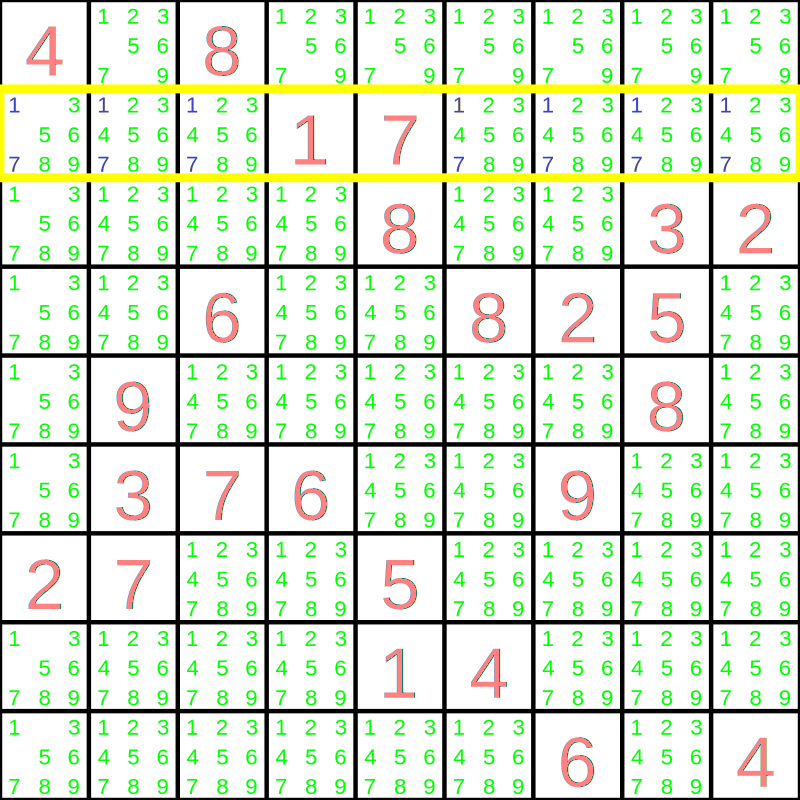
\includegraphics[width=6cm]{../sudoku/FC/frame4}}
\only<5>{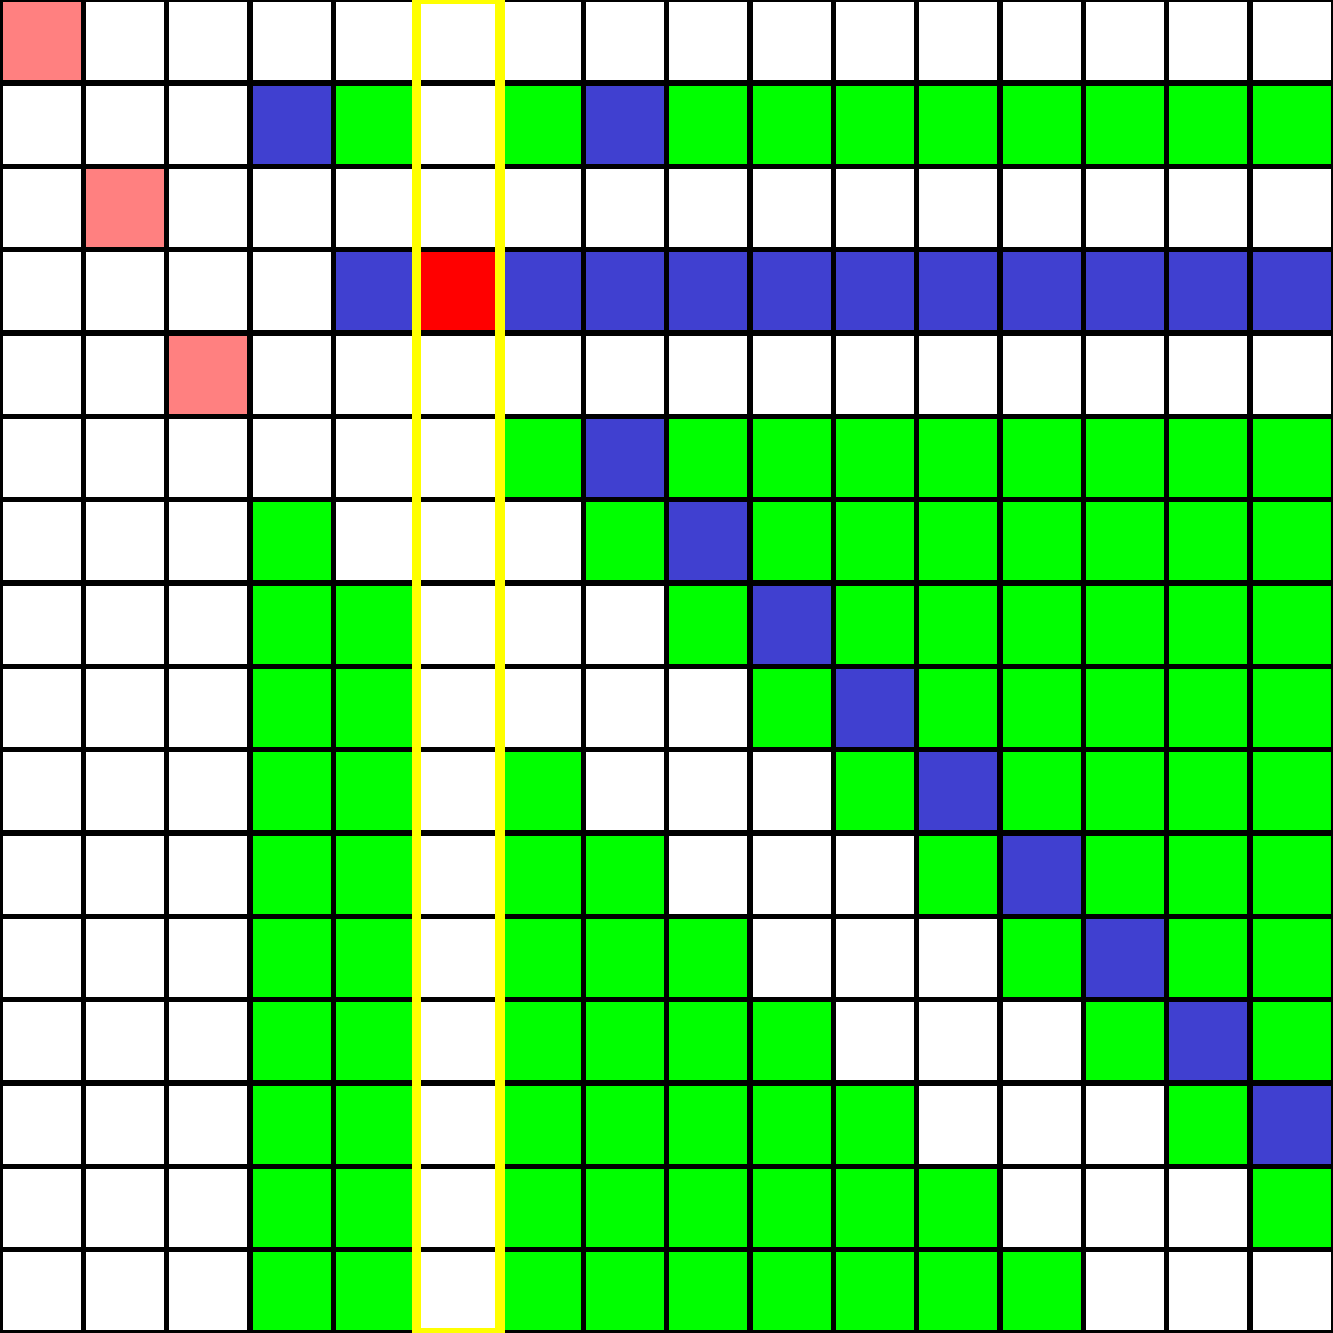
\includegraphics[width=6cm]{../sudoku/FC/frame5}}
\only<6>{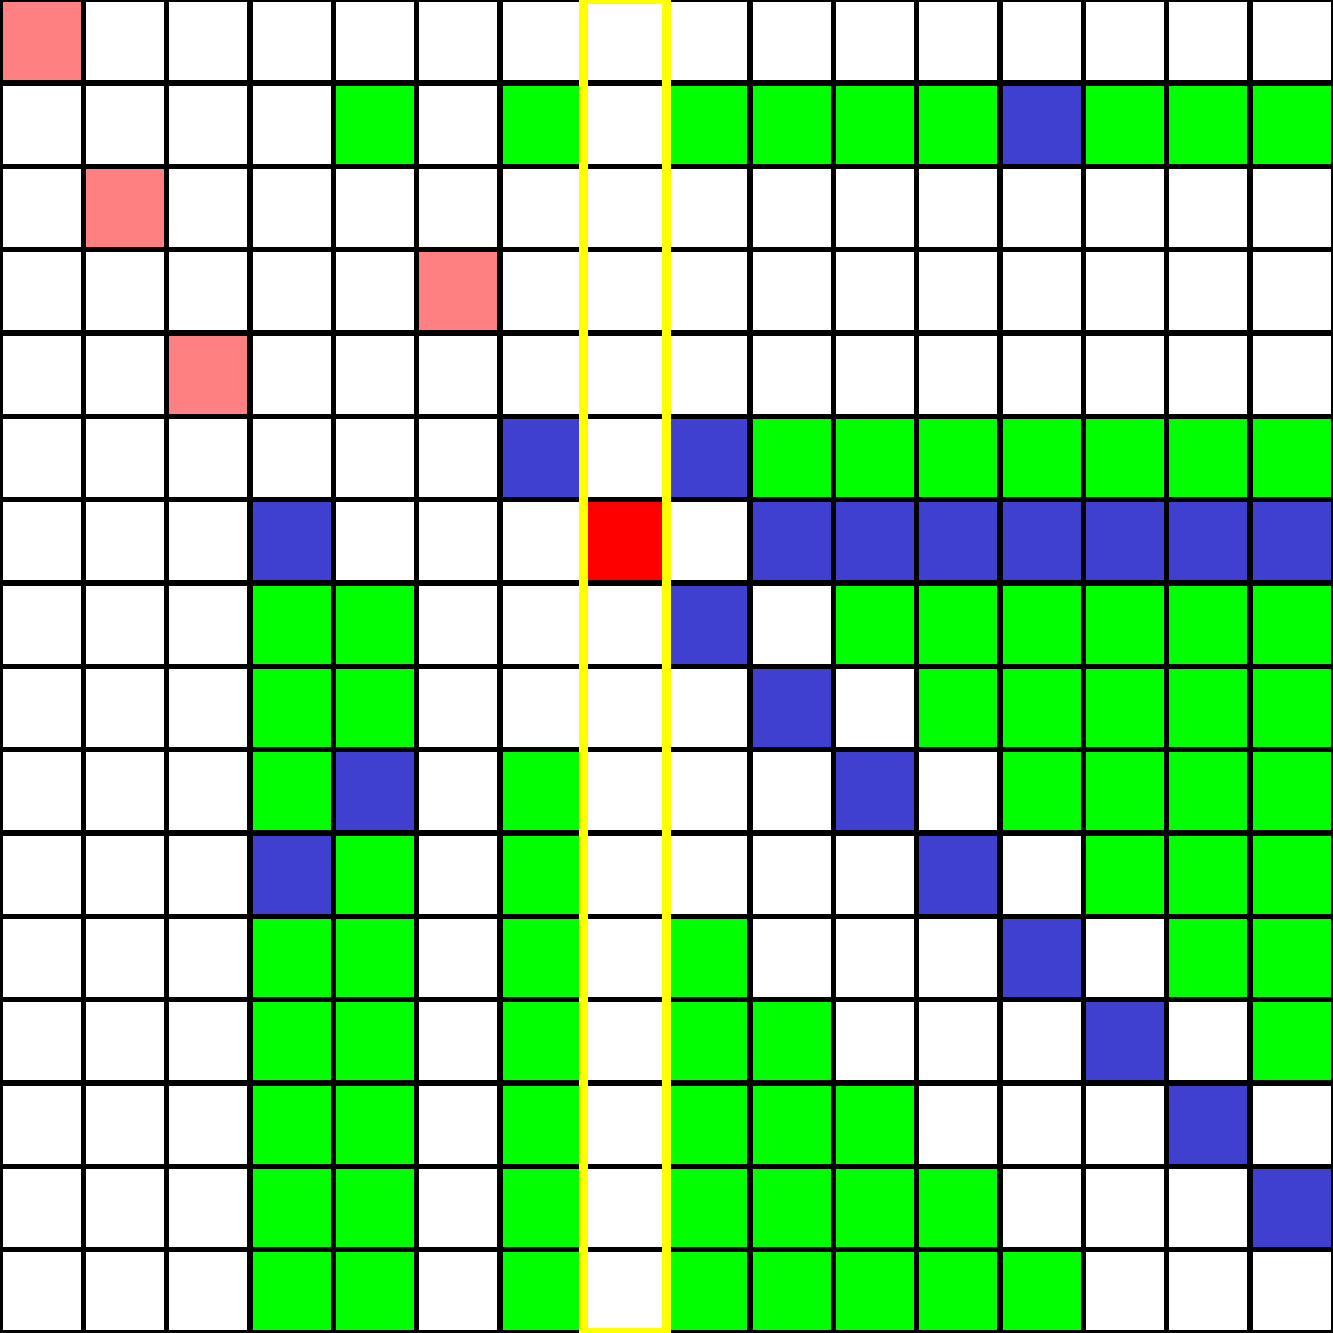
\includegraphics[width=6cm]{../sudoku/FC/frame6}}
\only<7>{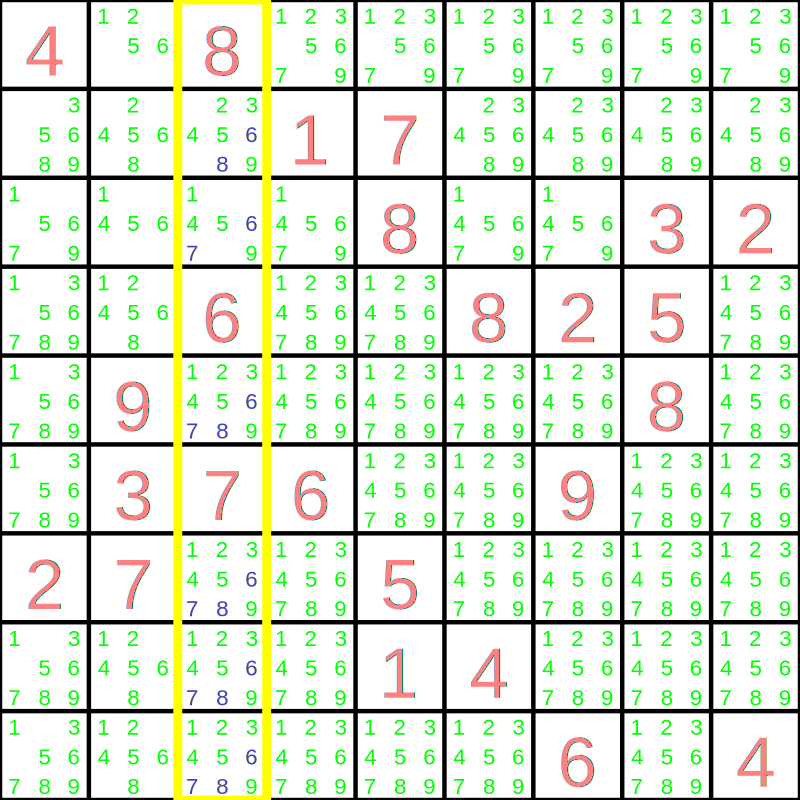
\includegraphics[width=6cm]{../sudoku/FC/frame7}}
\only<8>{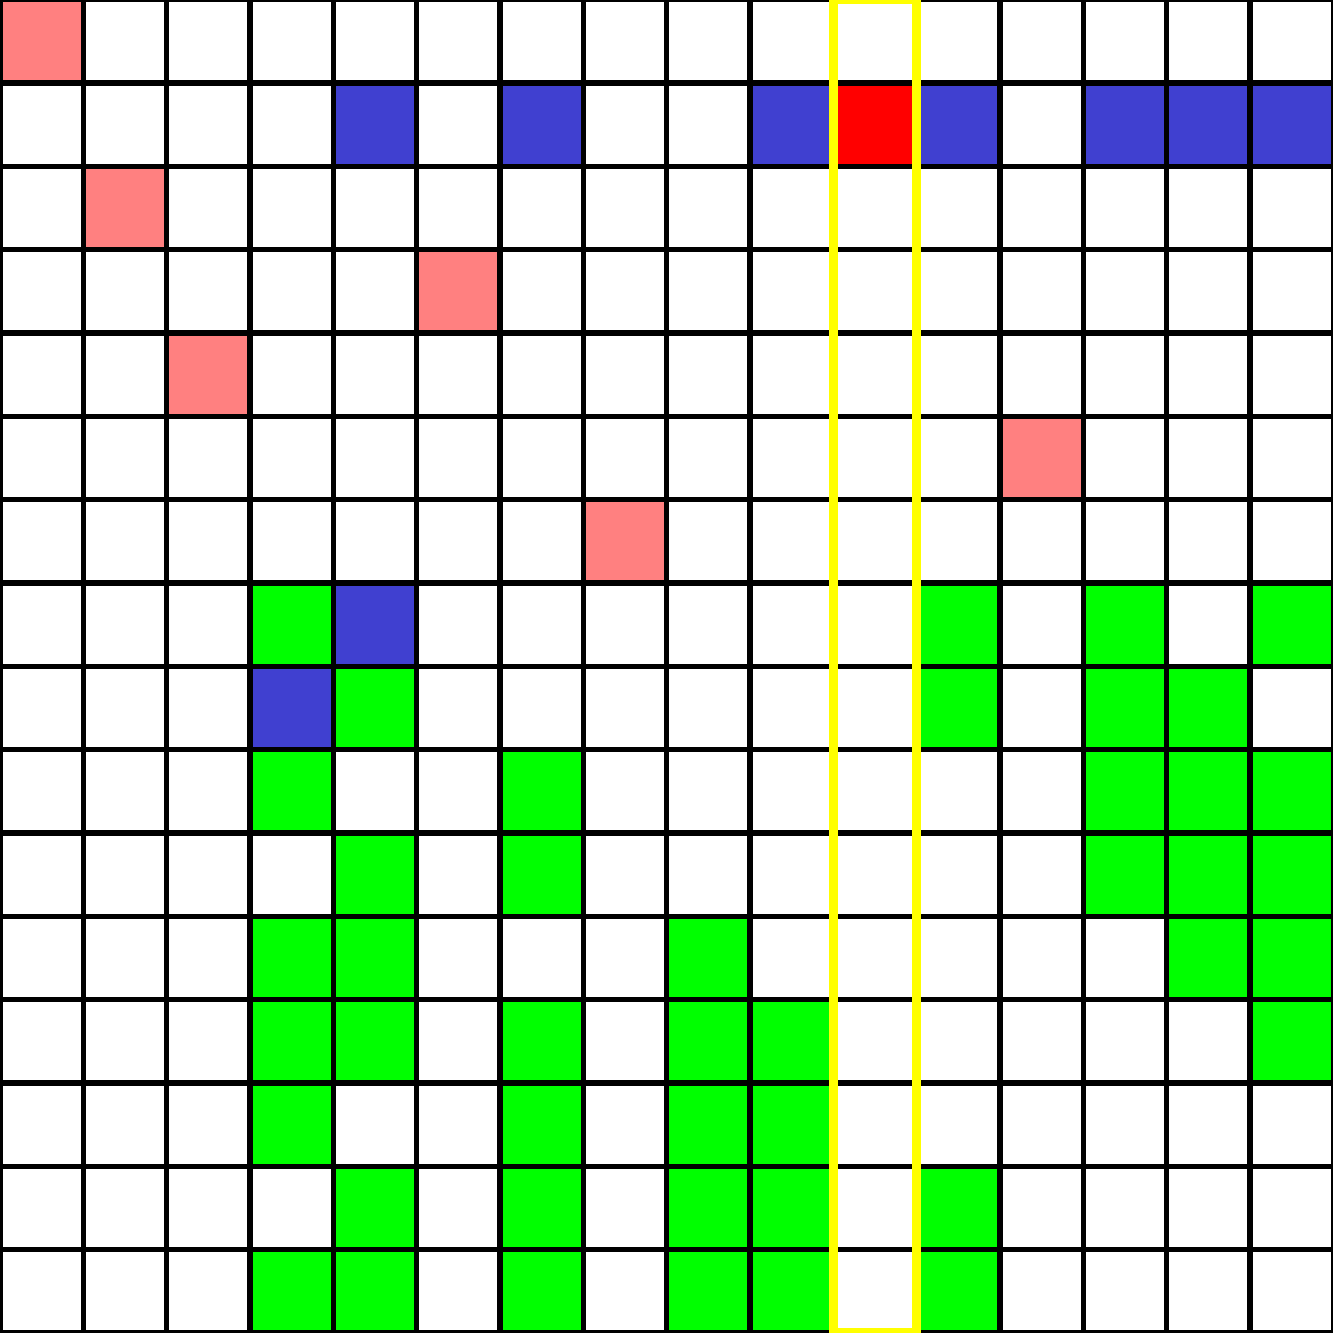
\includegraphics[width=6cm]{../sudoku/FC/frame8}}
\only<9>{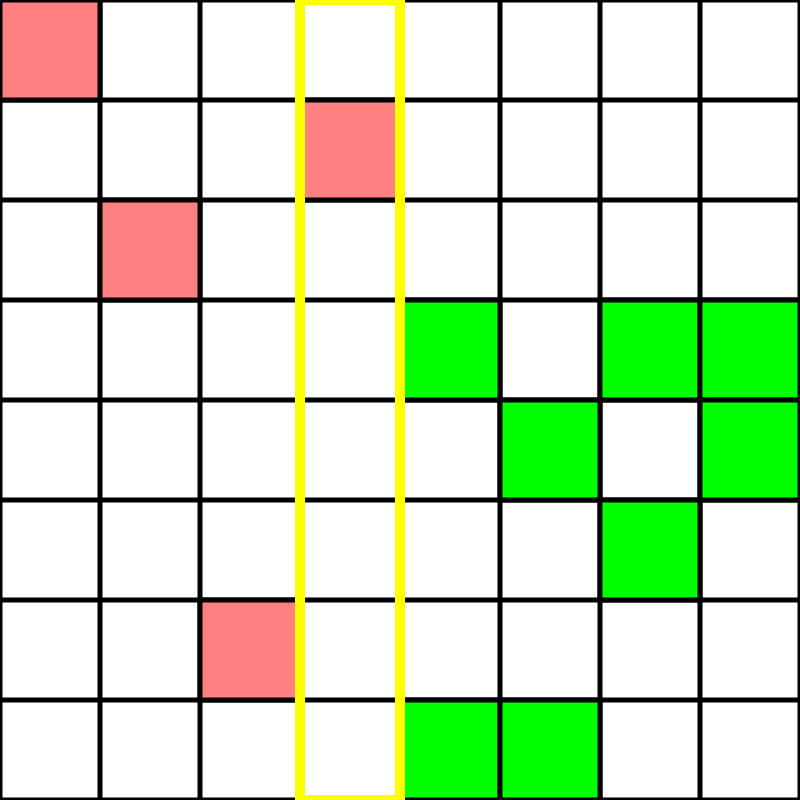
\includegraphics[width=6cm]{../sudoku/FC/frame9}}
\only<10>{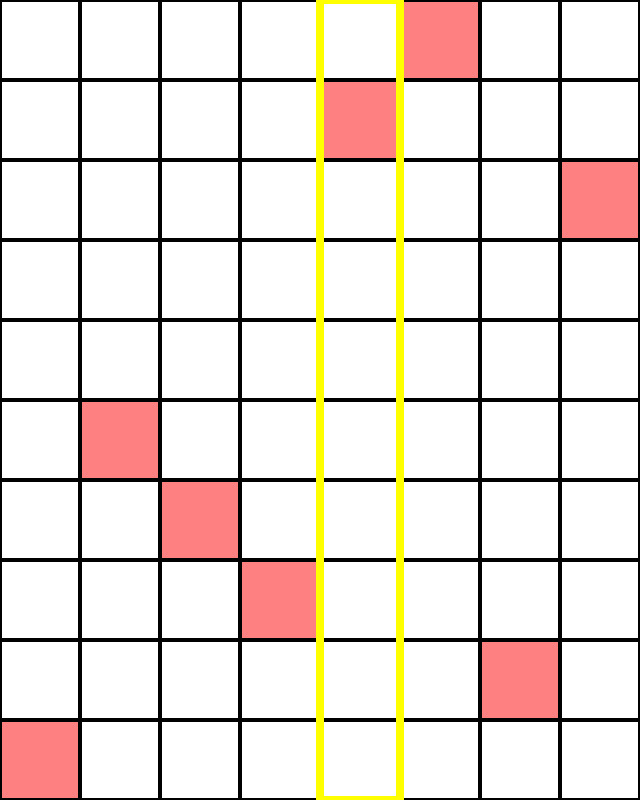
\includegraphics[width=6cm]{../sudoku/FC/frame10}}
\only<11>{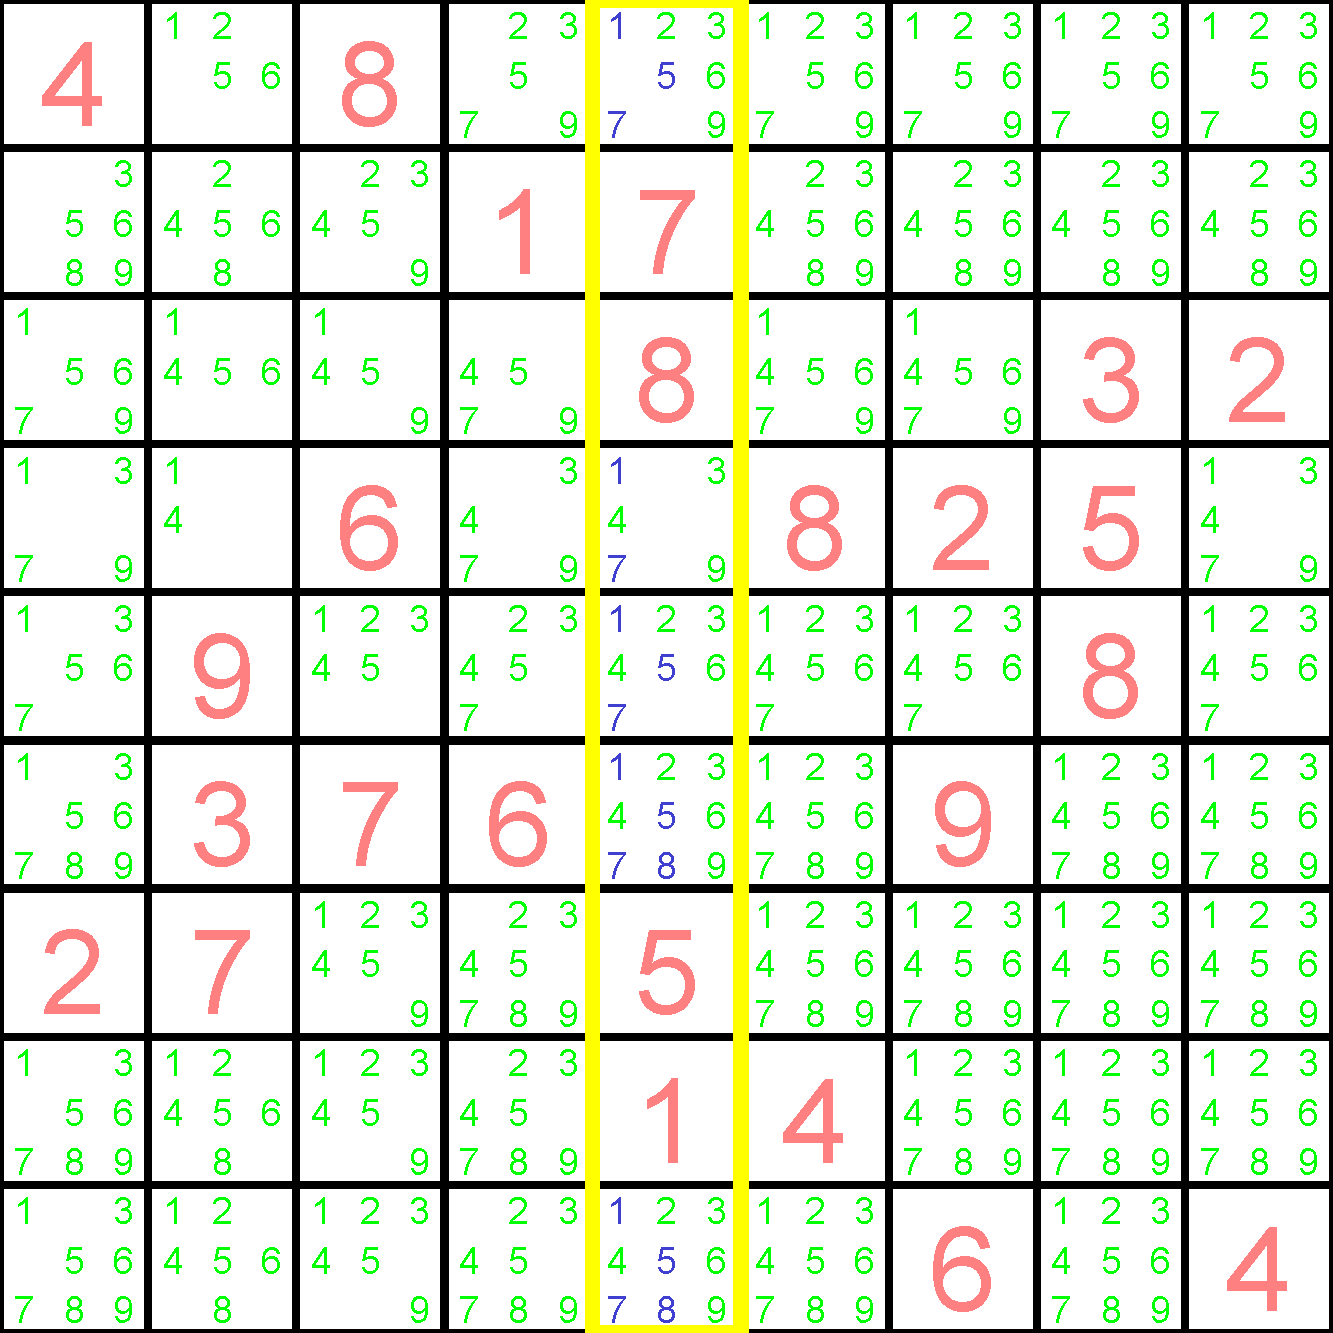
\includegraphics[width=6cm]{../sudoku/FC/frame11}}
\only<12>{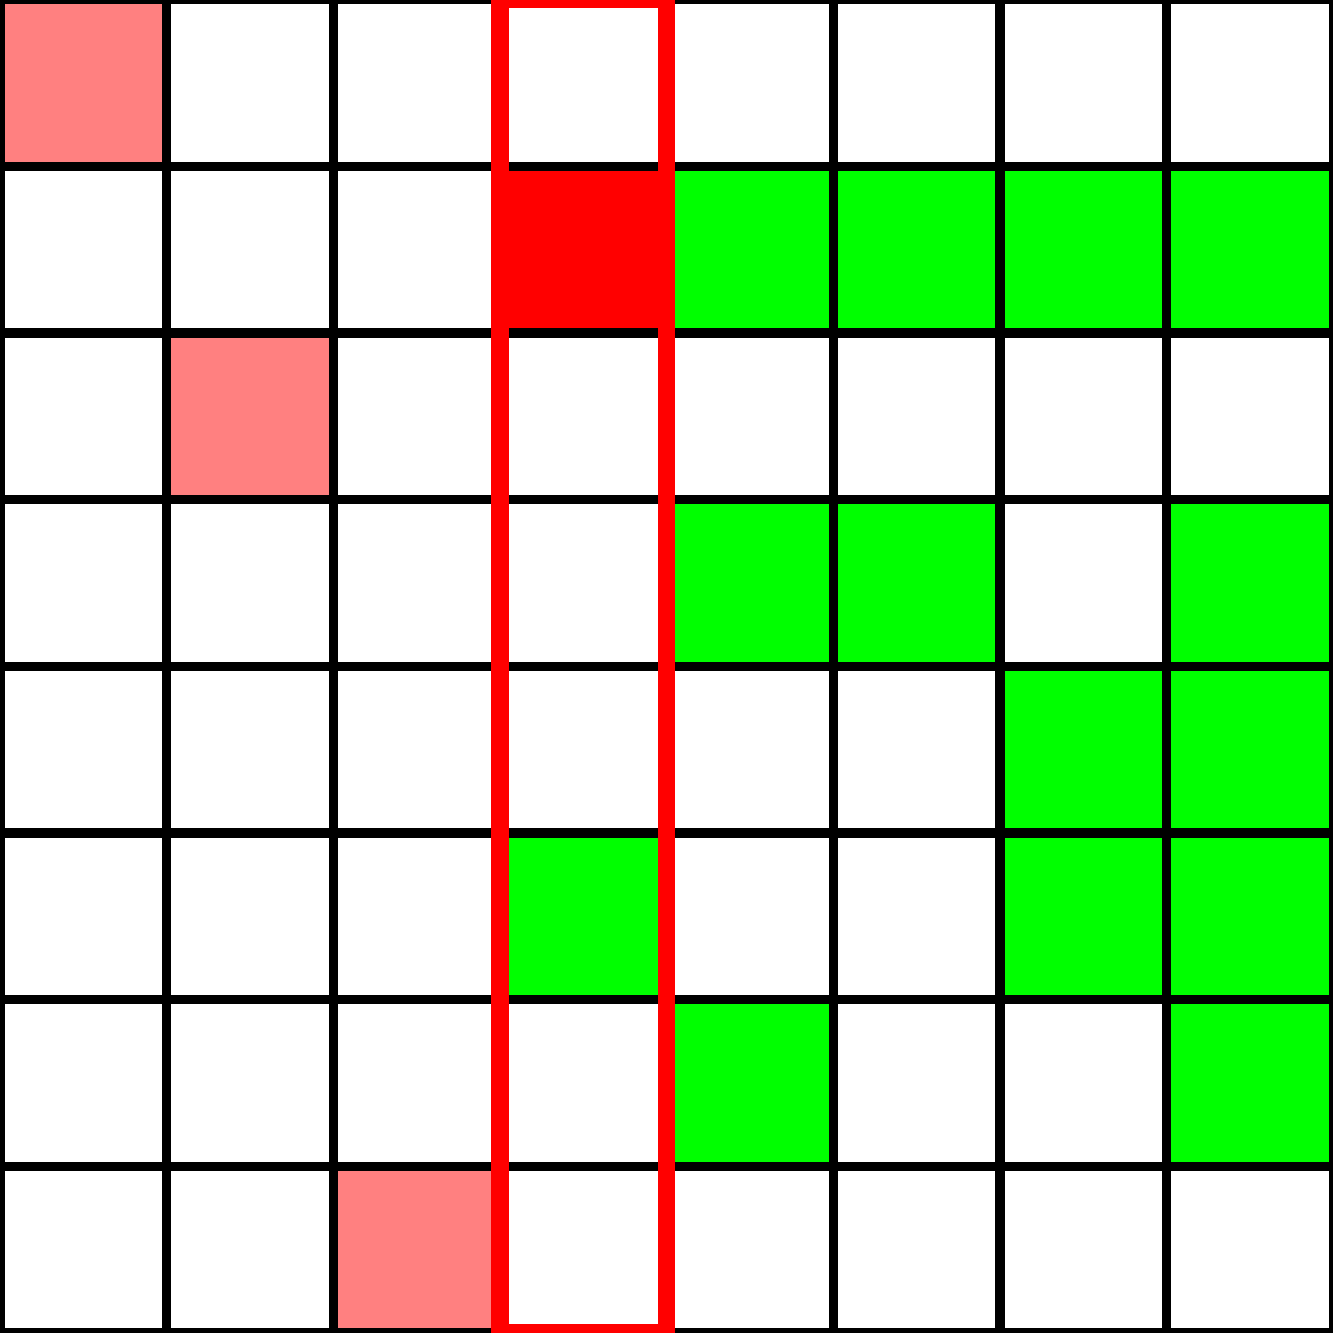
\includegraphics[width=6cm]{../sudoku/FC/frame12}}
\only<13>{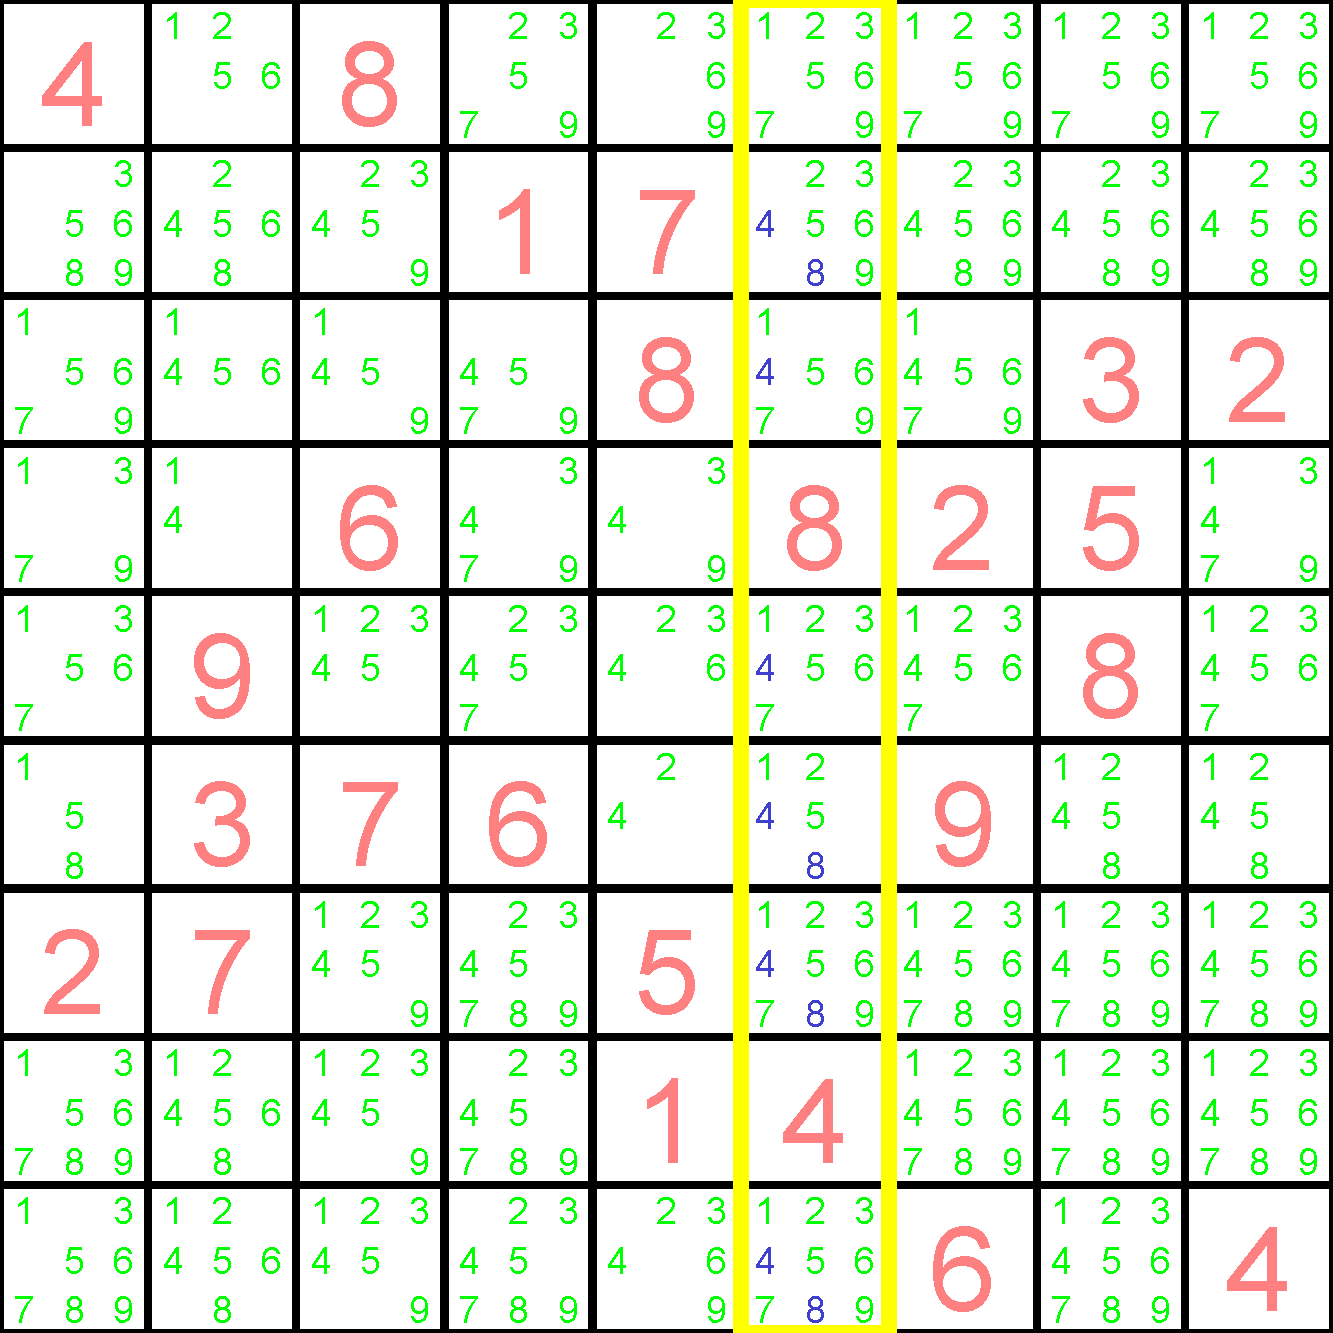
\includegraphics[width=6cm]{../sudoku/FC/frame13}}
\only<14>{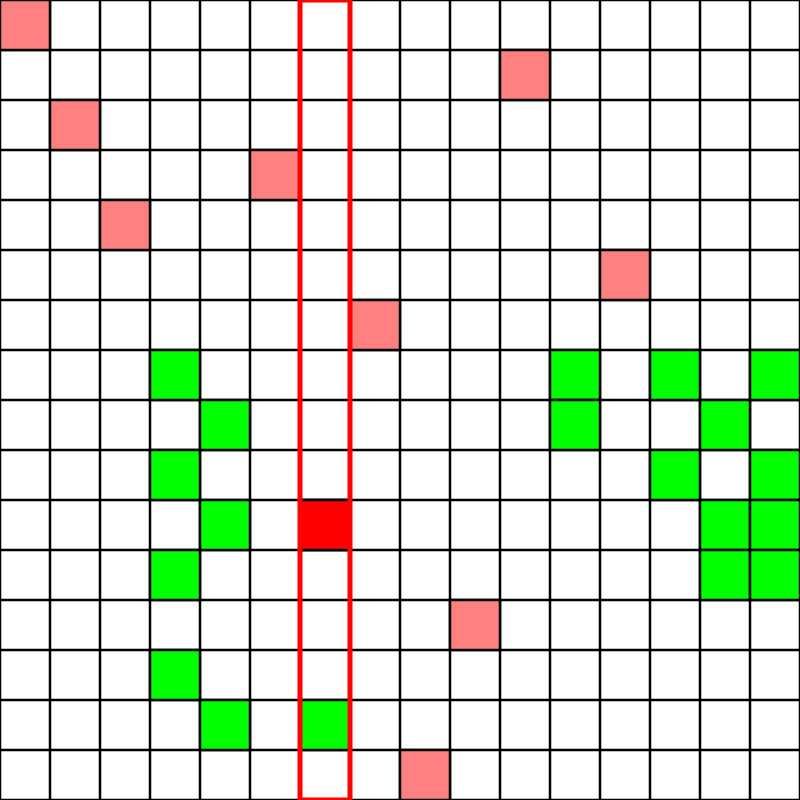
\includegraphics[width=6cm]{../sudoku/FC/frame14}}
\only<15>{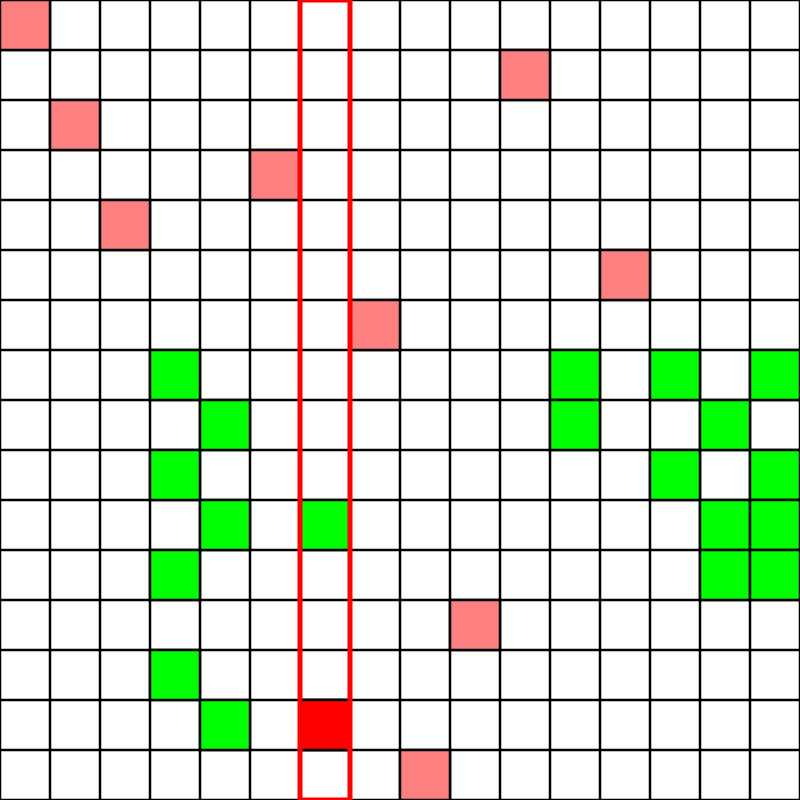
\includegraphics[width=6cm]{../sudoku/FC/frame15}}
\only<16>{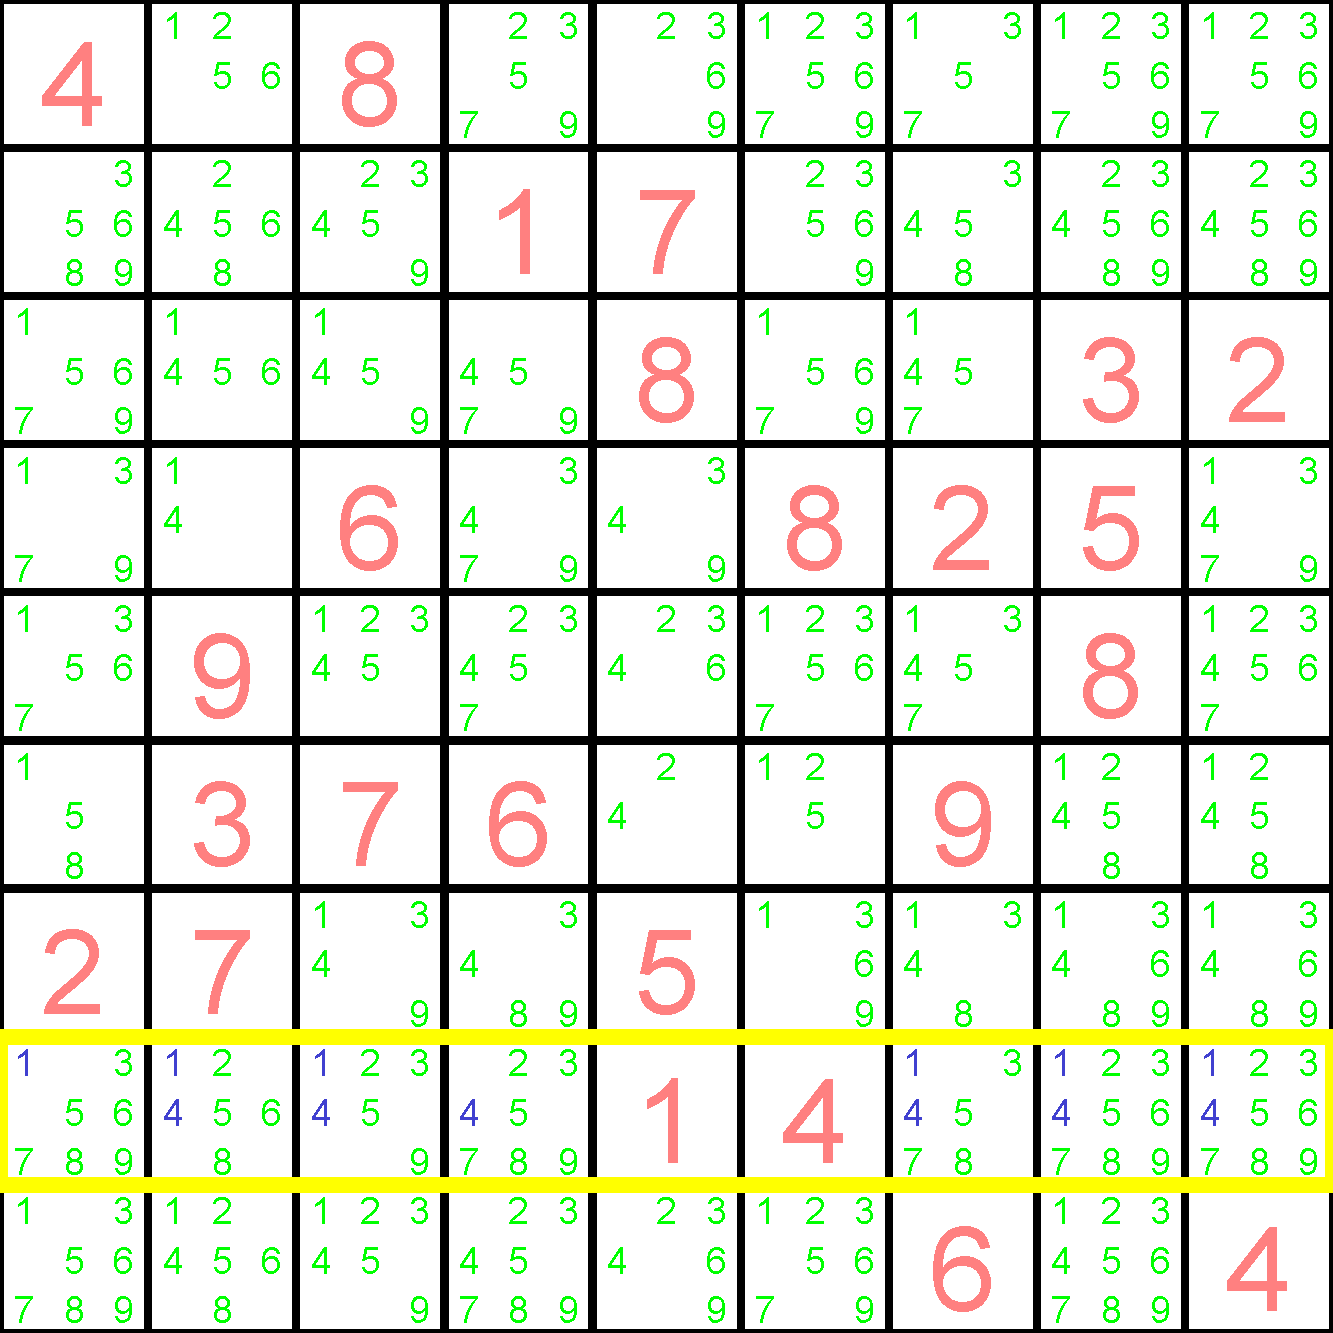
\includegraphics[width=6cm]{../sudoku/FC/frame16}}
\only<17>{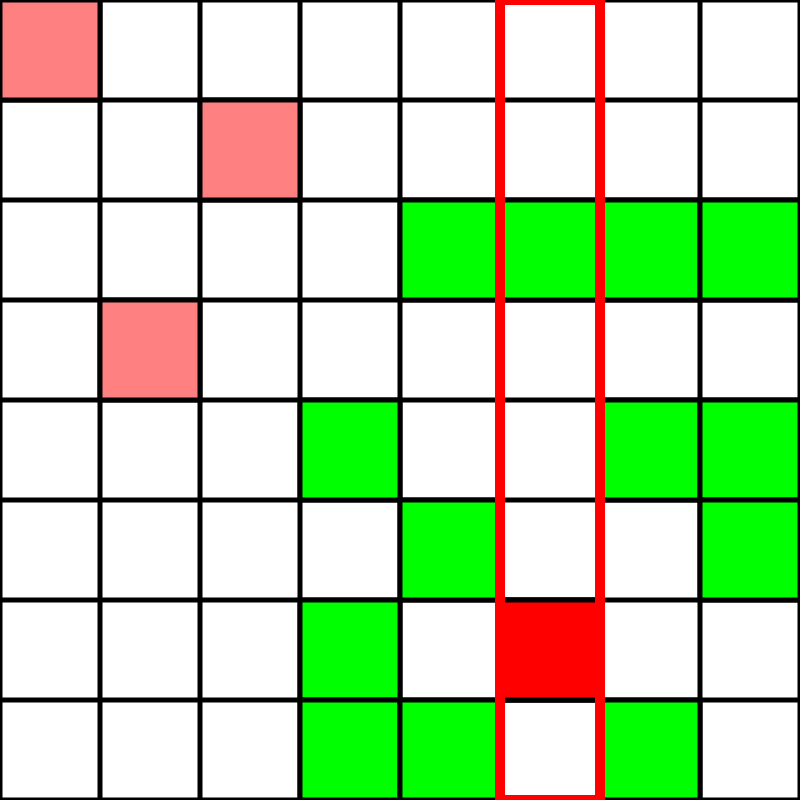
\includegraphics[width=6cm]{../sudoku/FC/frame17}}
\only<18>{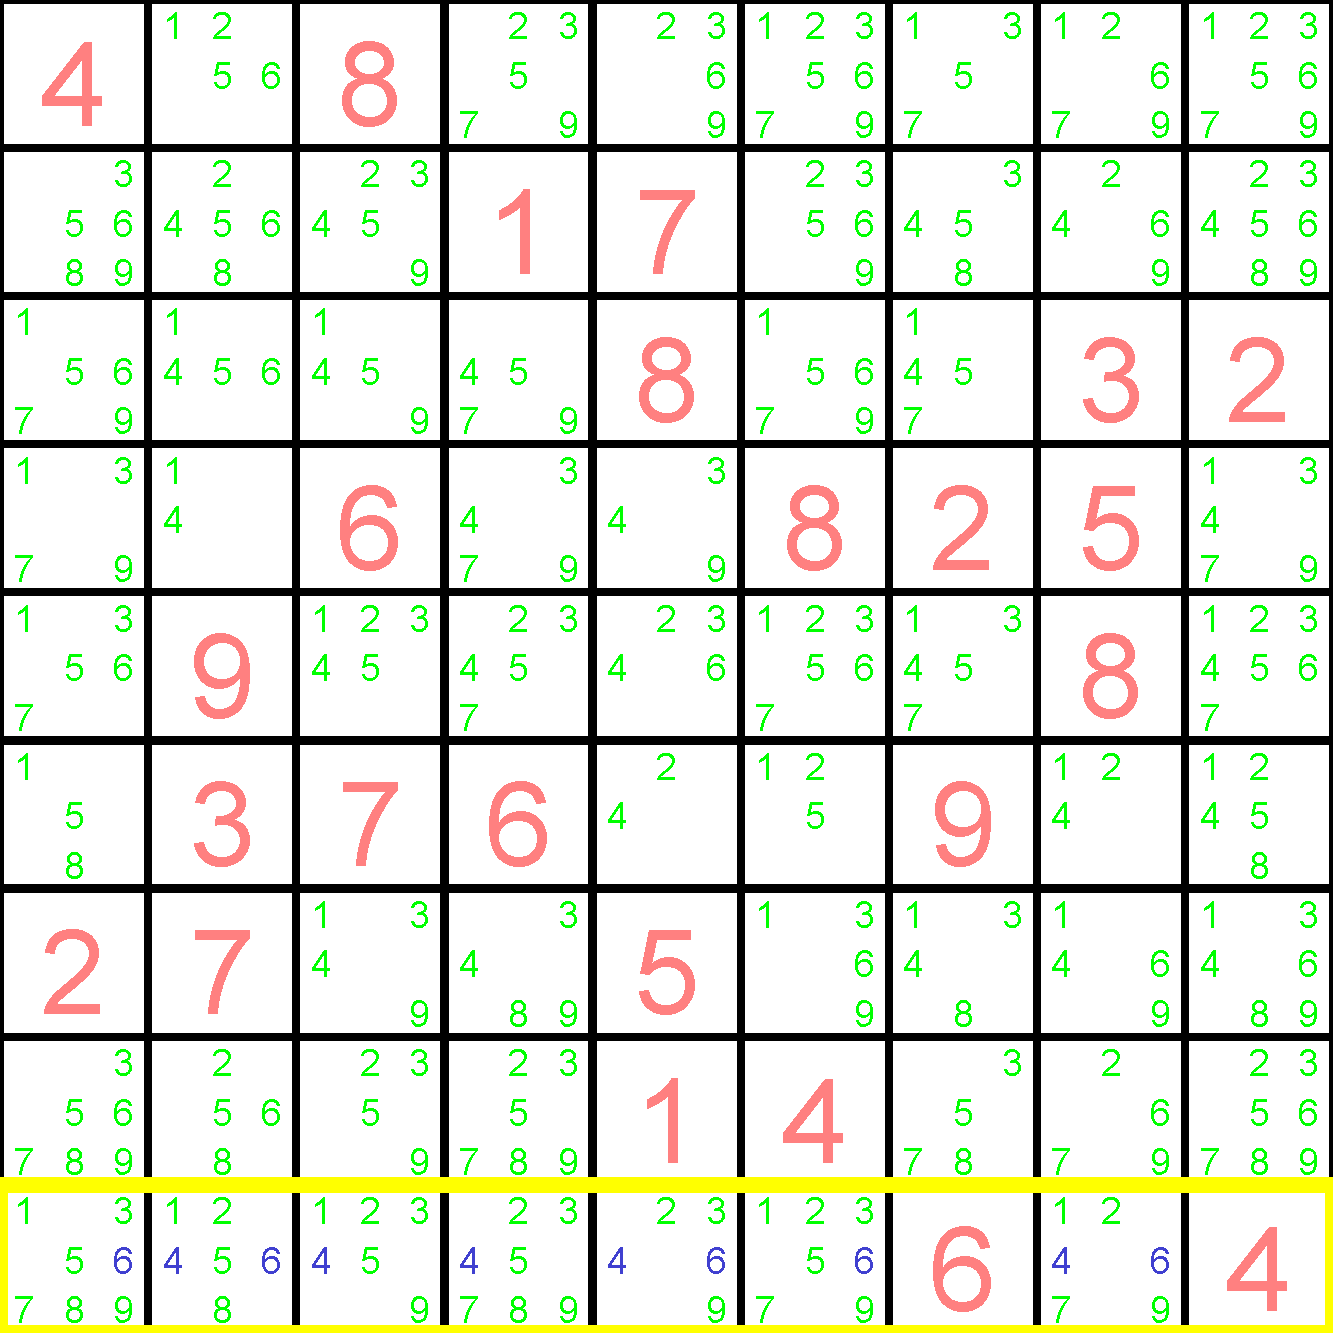
\includegraphics[width=6cm]{../sudoku/FC/frame18}}
\only<19>{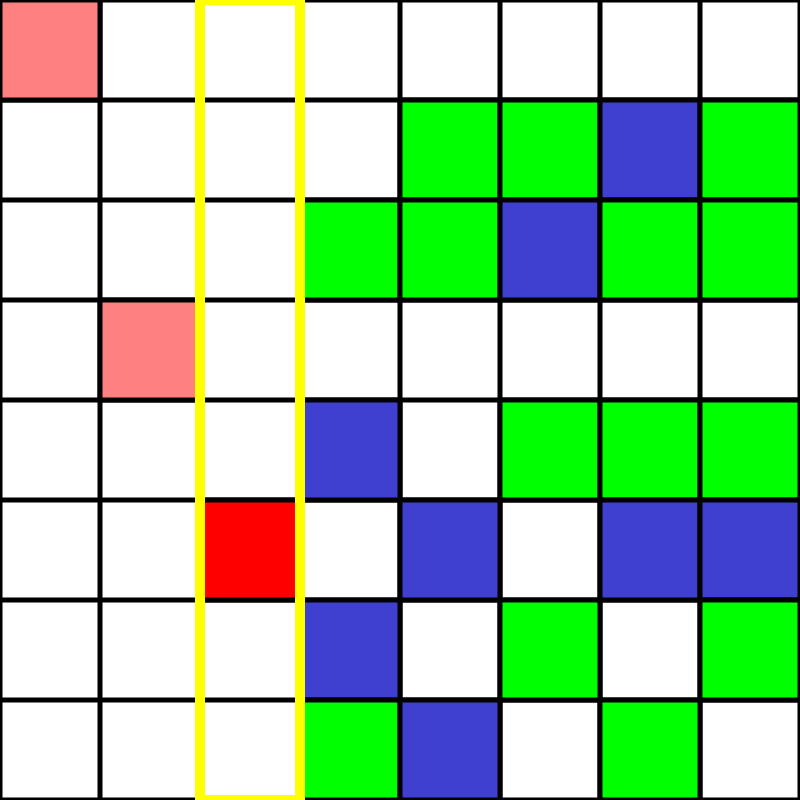
\includegraphics[width=6cm]{../sudoku/FC/frame19}}
\only<20>{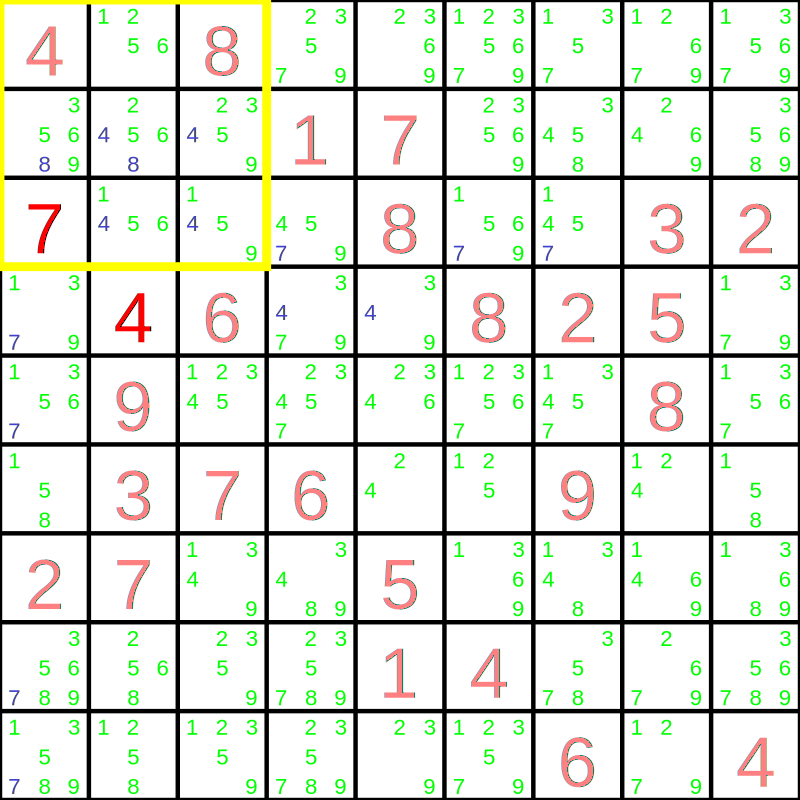
\includegraphics[width=6cm]{../sudoku/FC/frame20}}
\only<21>{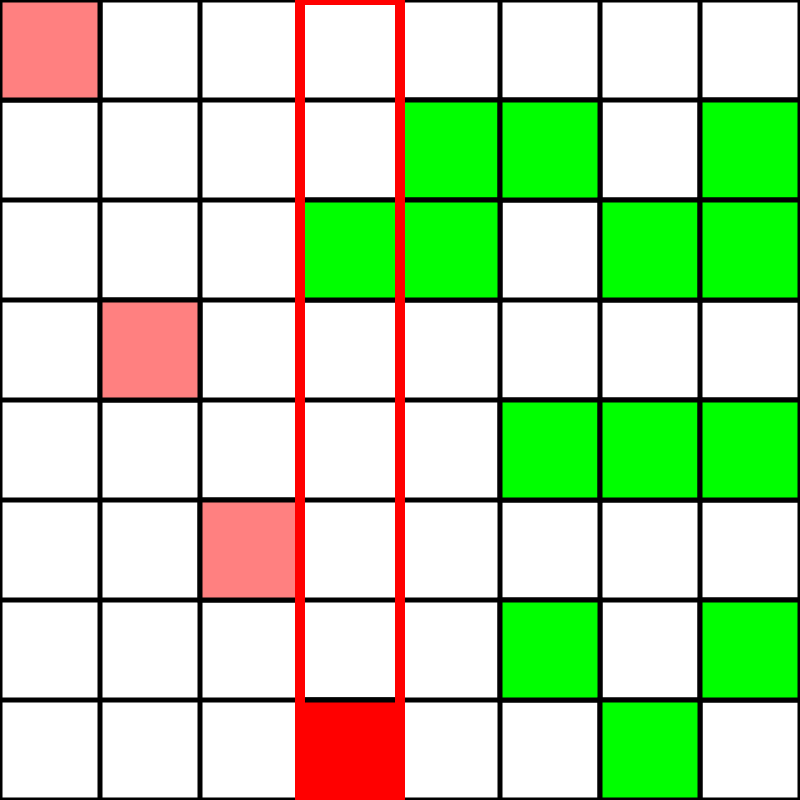
\includegraphics[width=6cm]{../sudoku/FC/frame21}}
\only<22>{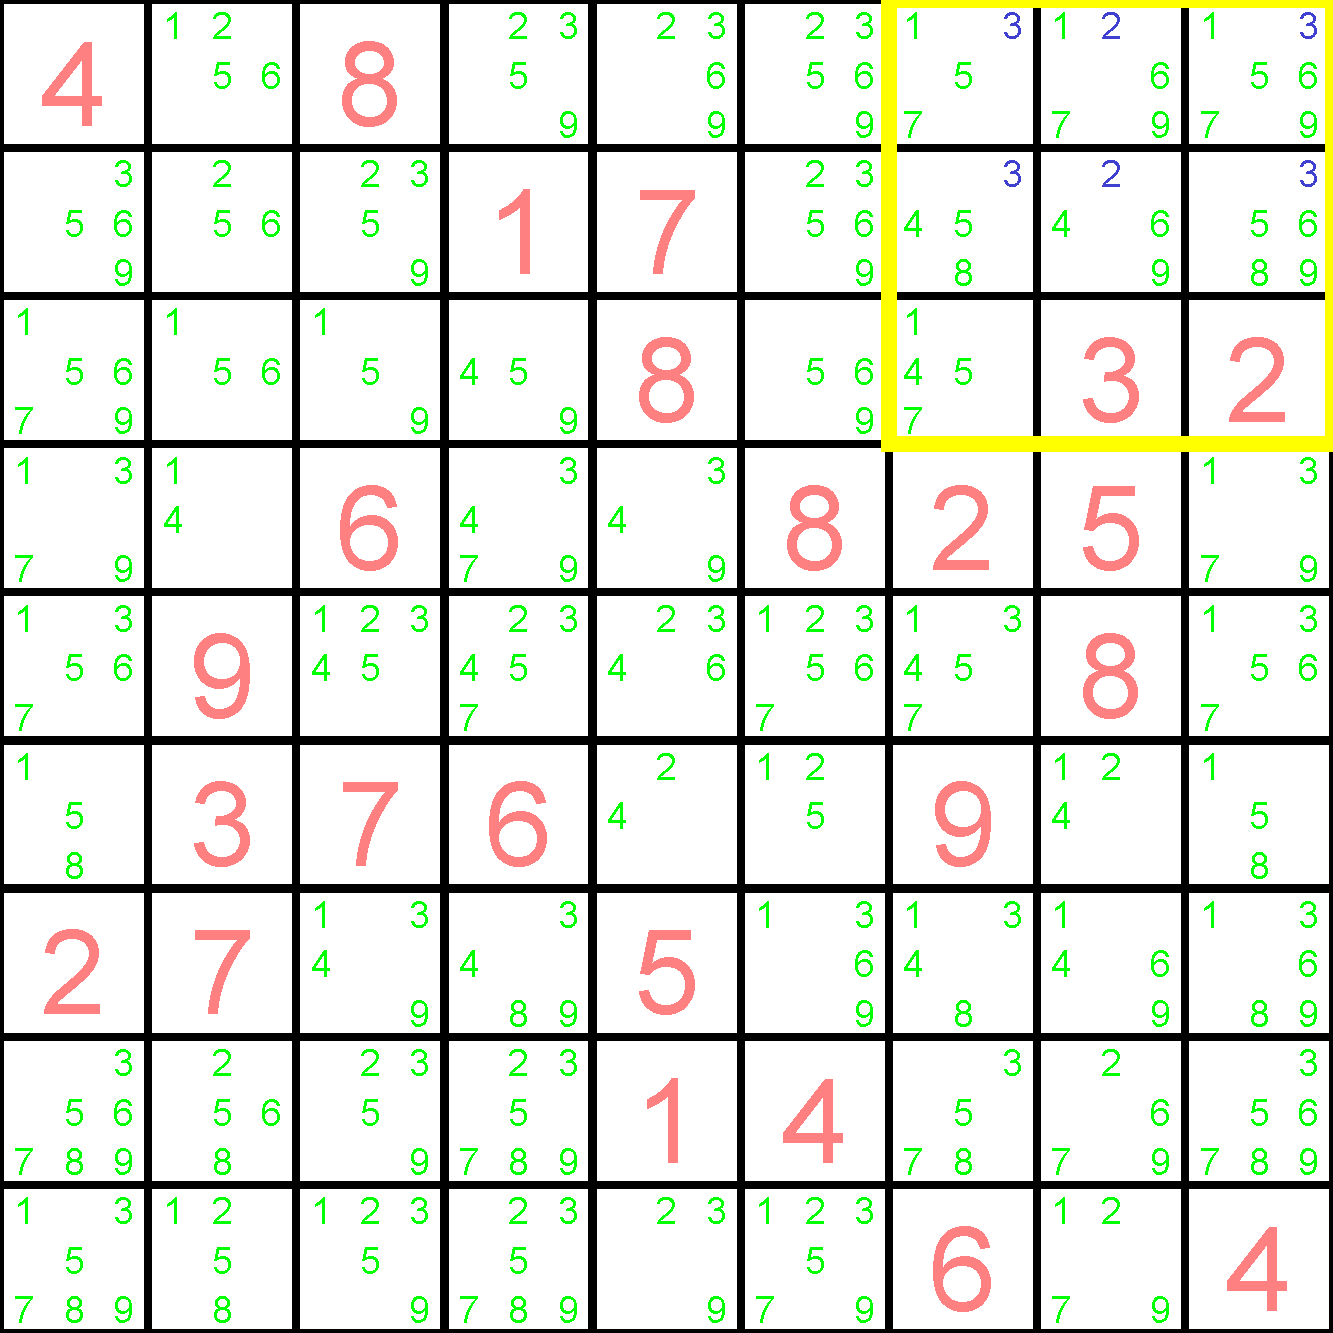
\includegraphics[width=6cm]{../sudoku/FC/frame22}}
\only<23>{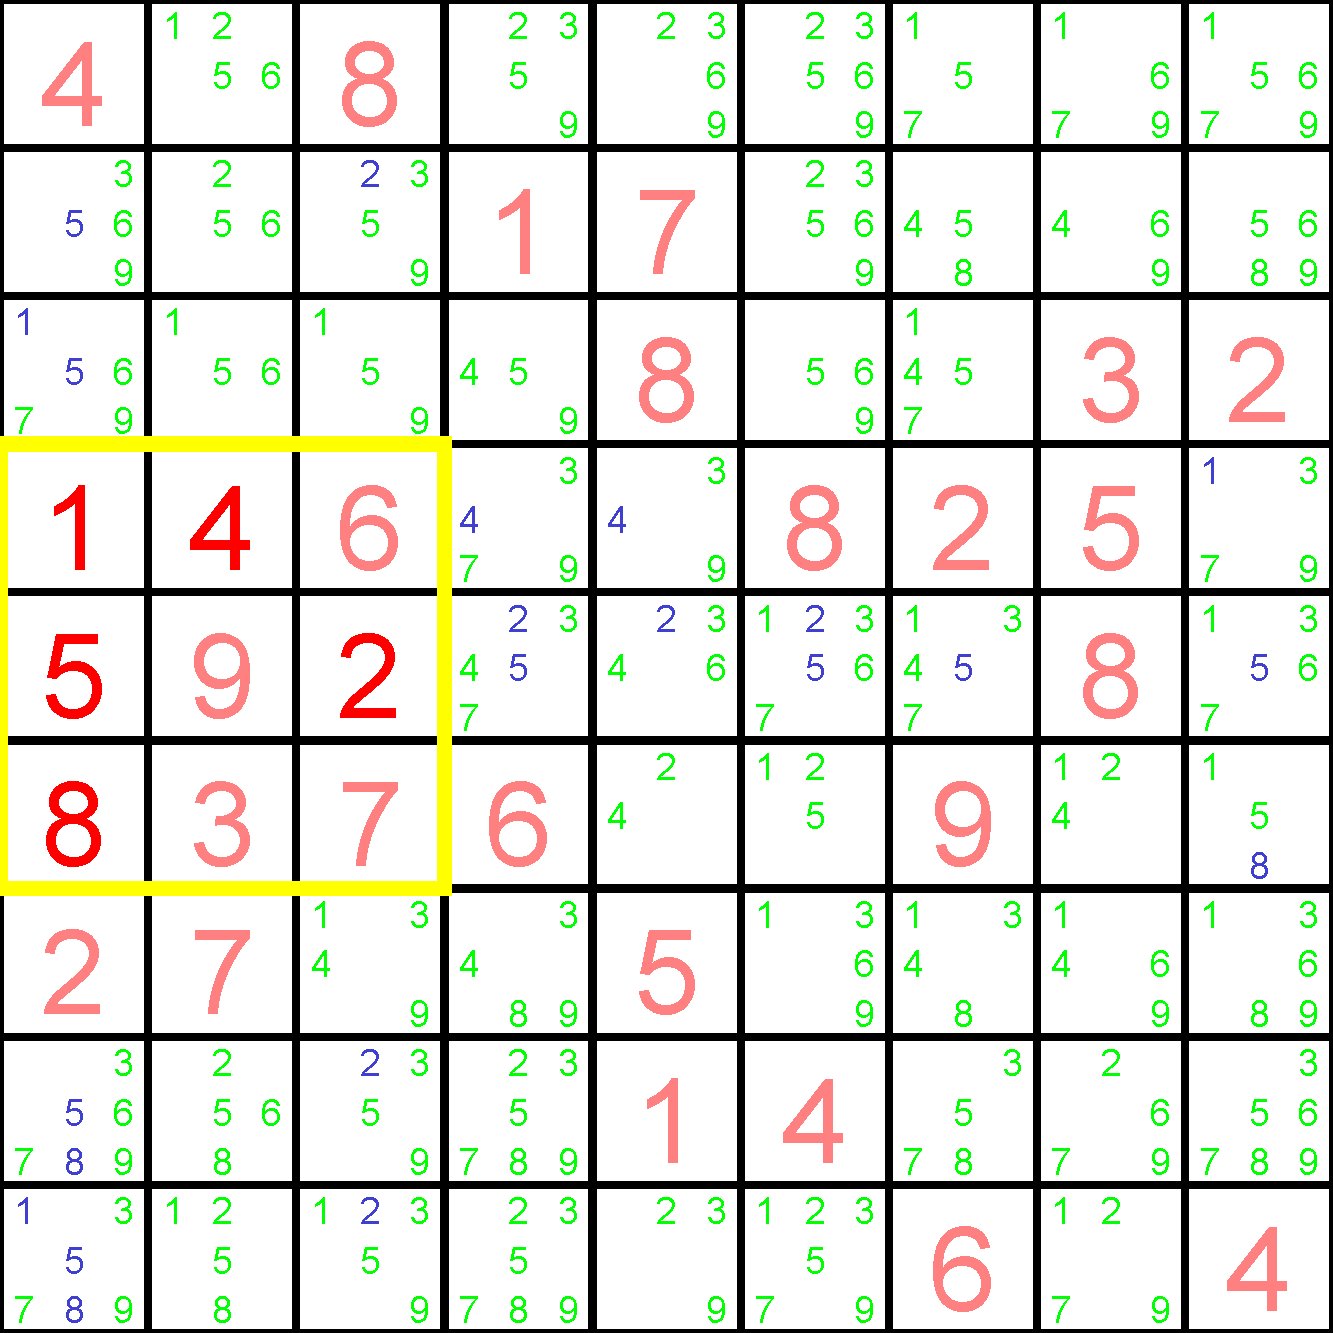
\includegraphics[width=6cm]{../sudoku/FC/frame23}}
\only<24>{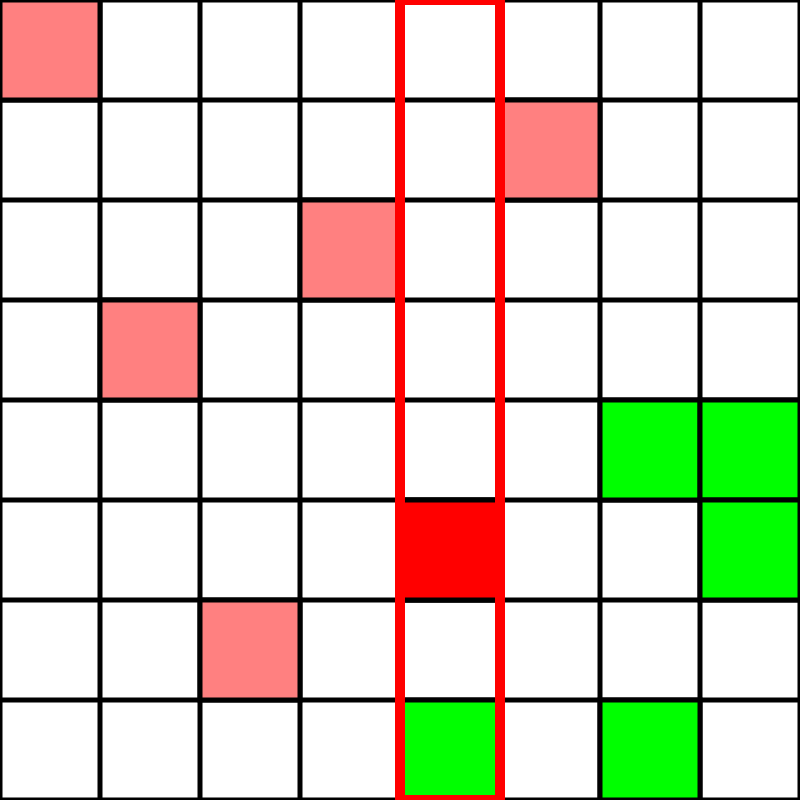
\includegraphics[width=6cm]{../sudoku/FC/frame24}}
\only<25>{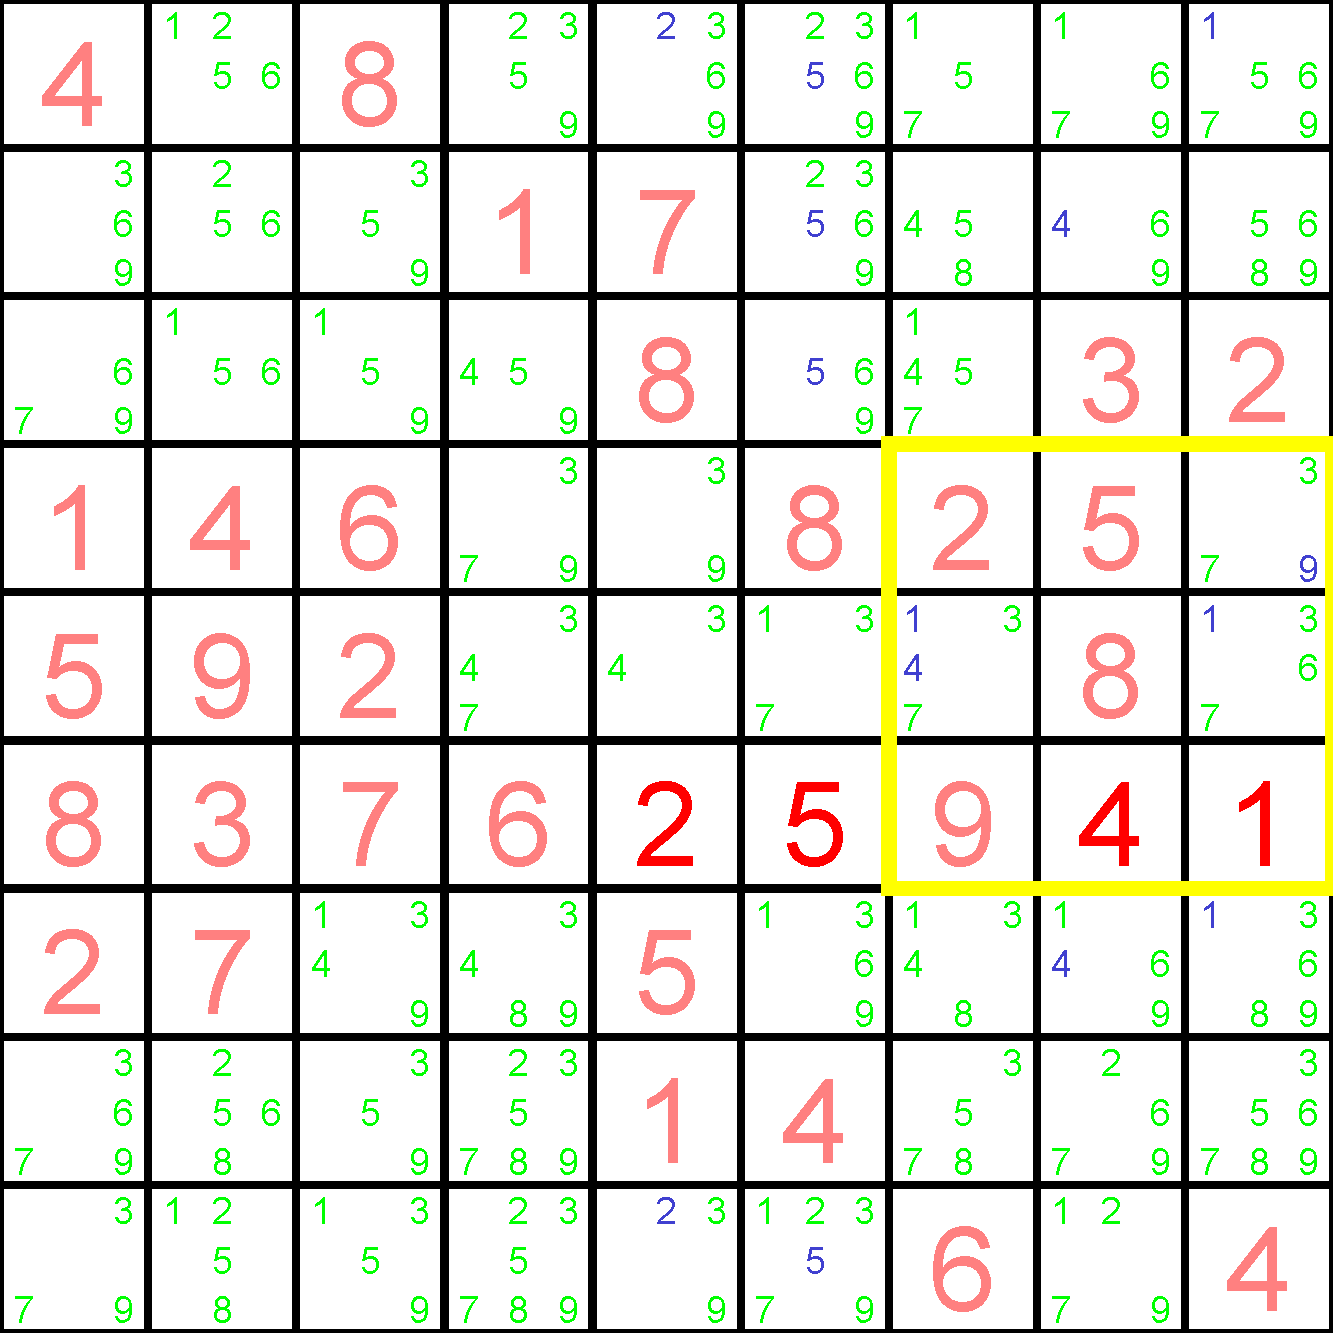
\includegraphics[width=6cm]{../sudoku/FC/frame25}}
\only<26>{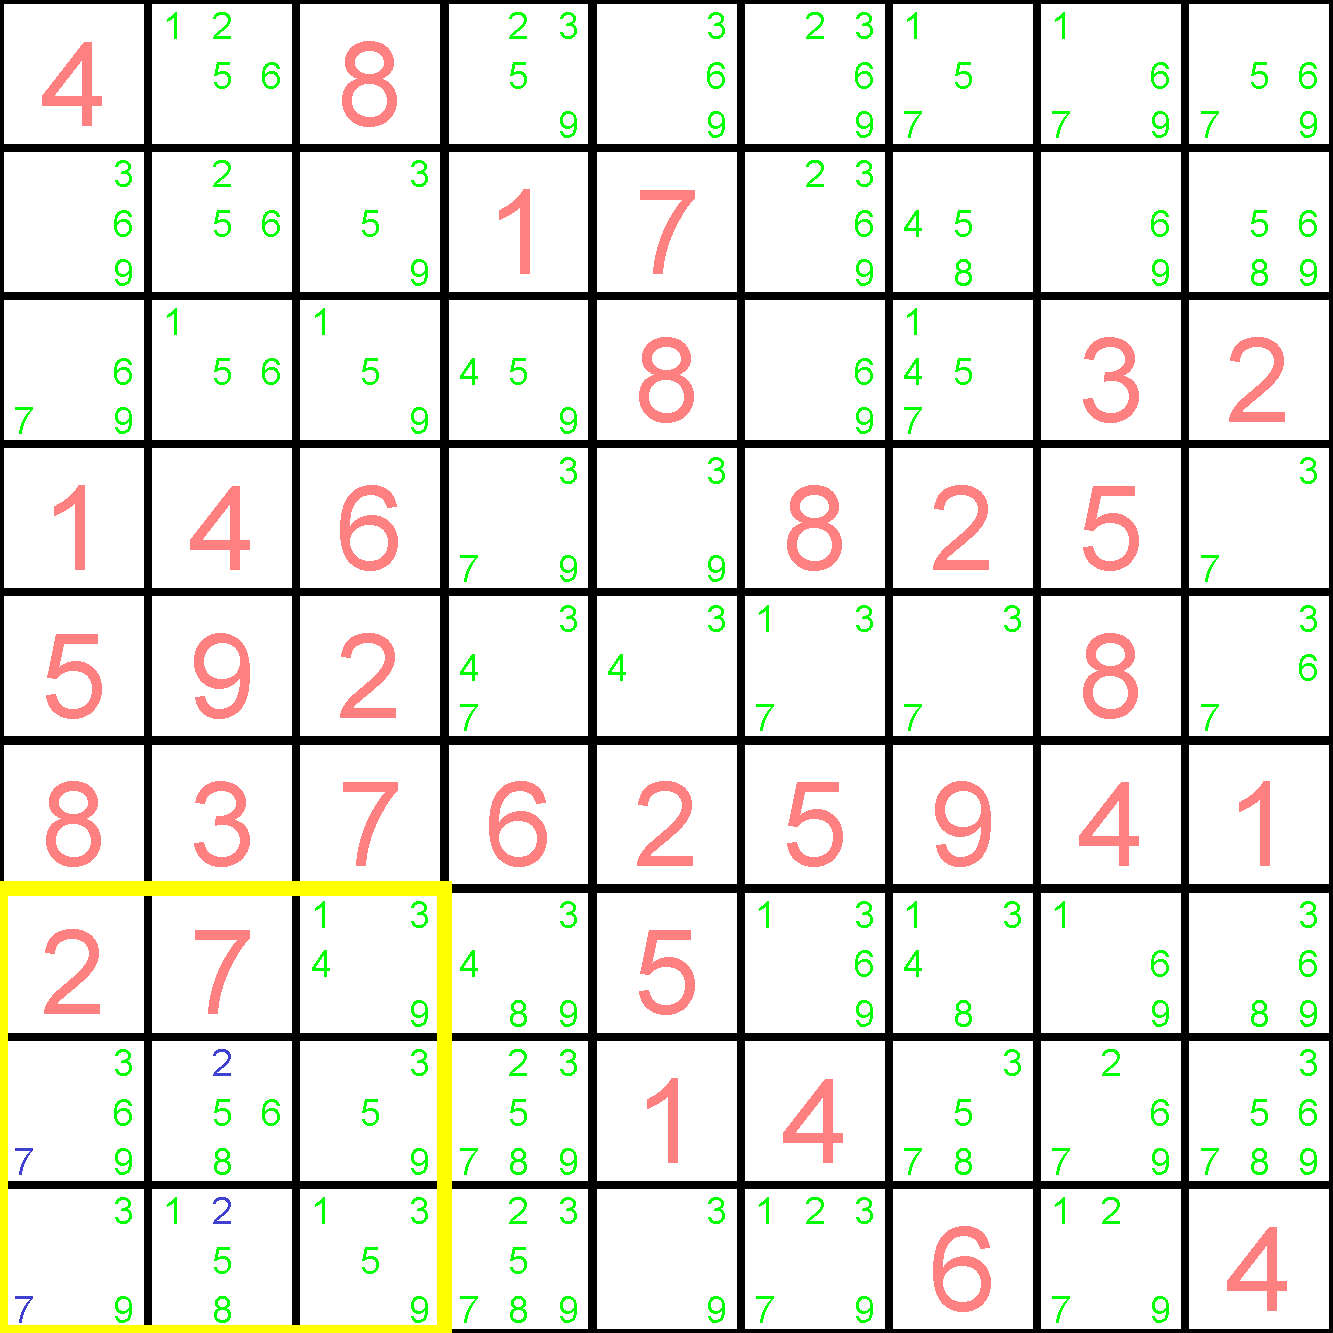
\includegraphics[width=6cm]{../sudoku/FC/frame26}}
\only<27>{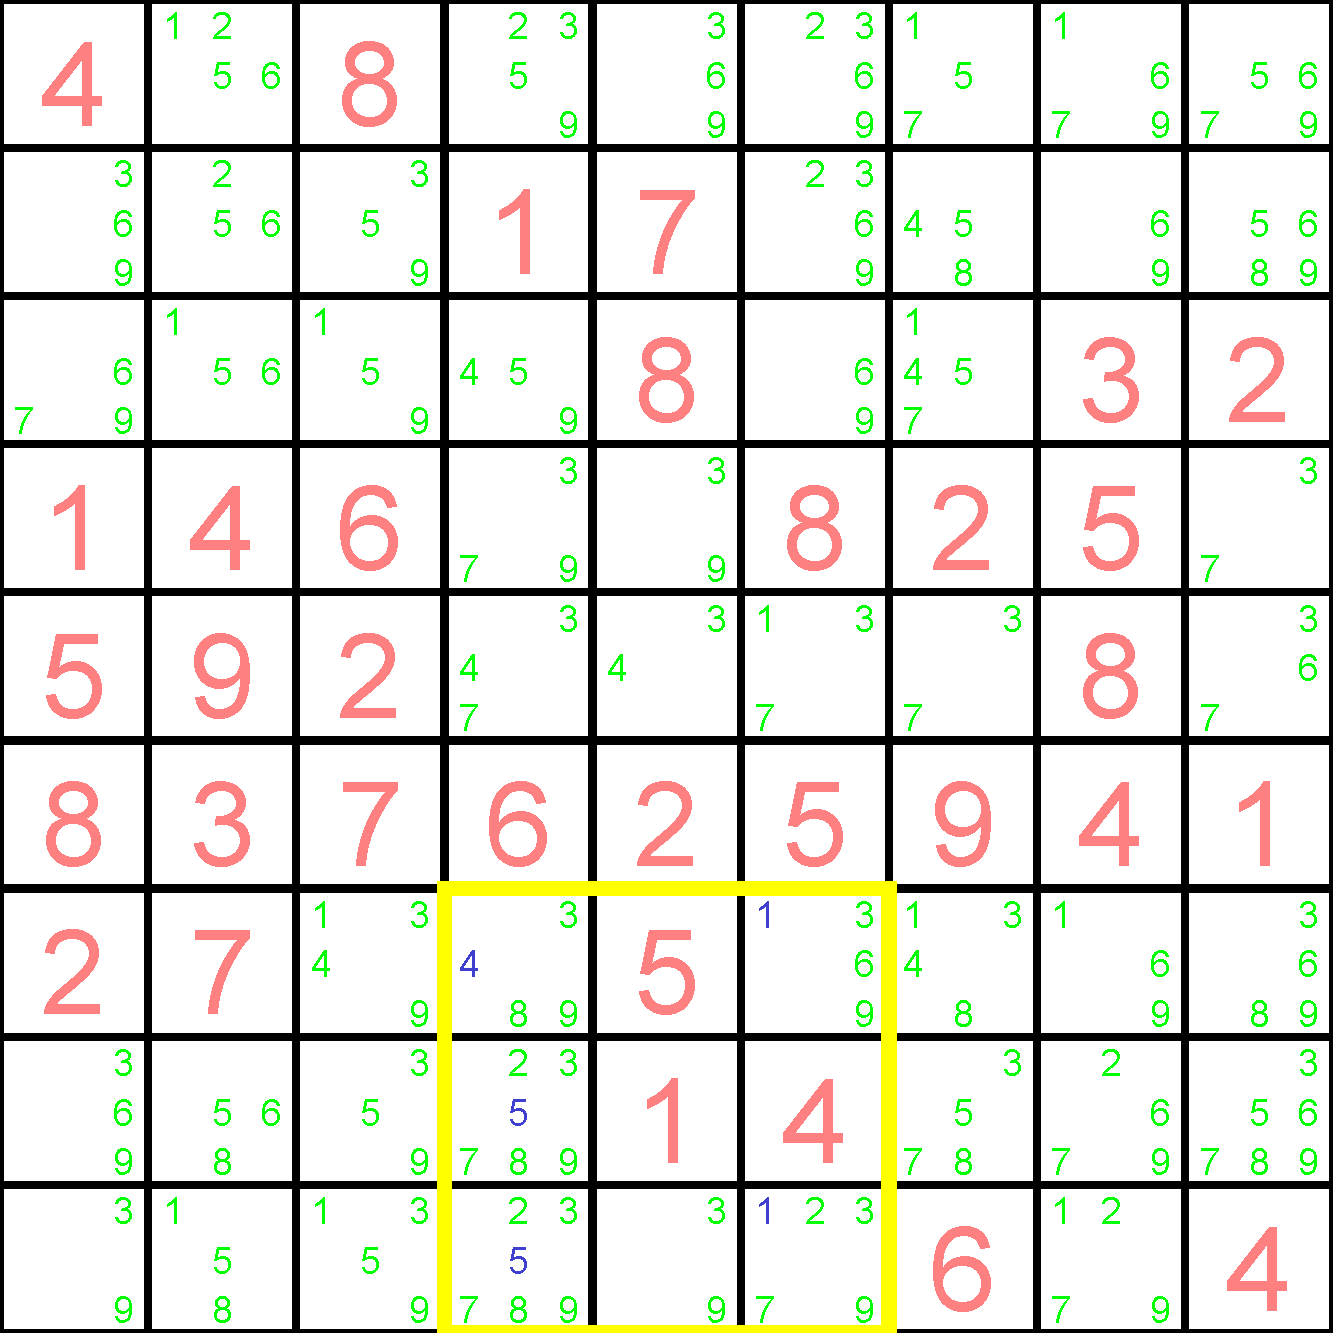
\includegraphics[width=6cm]{../sudoku/FC/frame27}}
\only<28>{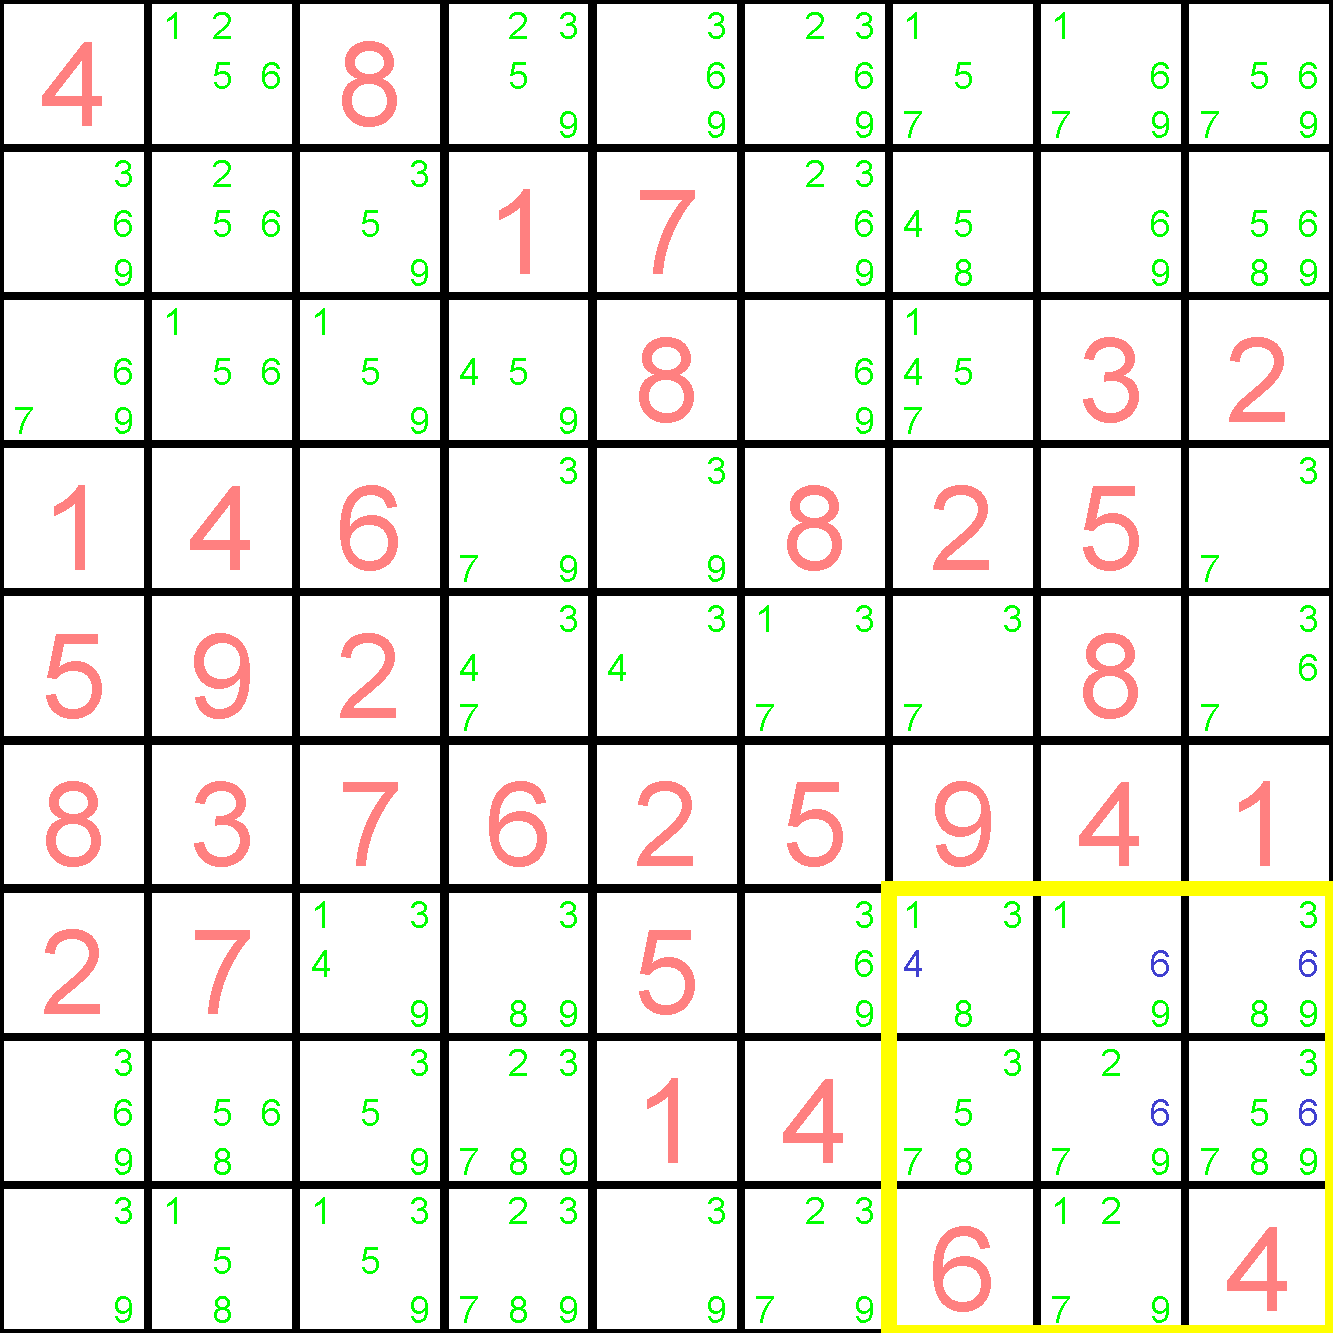
\includegraphics[width=6cm]{../sudoku/FC/frame28}}
\only<29>{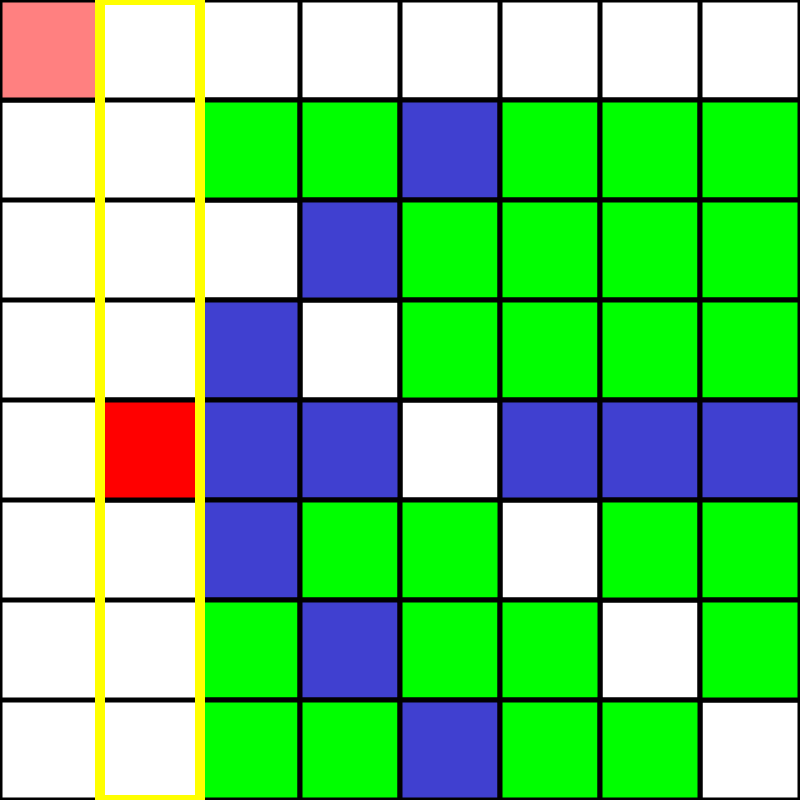
\includegraphics[width=6cm]{../sudoku/FC/frame29}}
\vfill
\hyperlinkframestart<2-29>{\beamerreturnbutton{Back to Start}}
\hyperlinkframeend<1-28>{\beamerskipbutton{Skip Animation}}
}
\only<handout>{
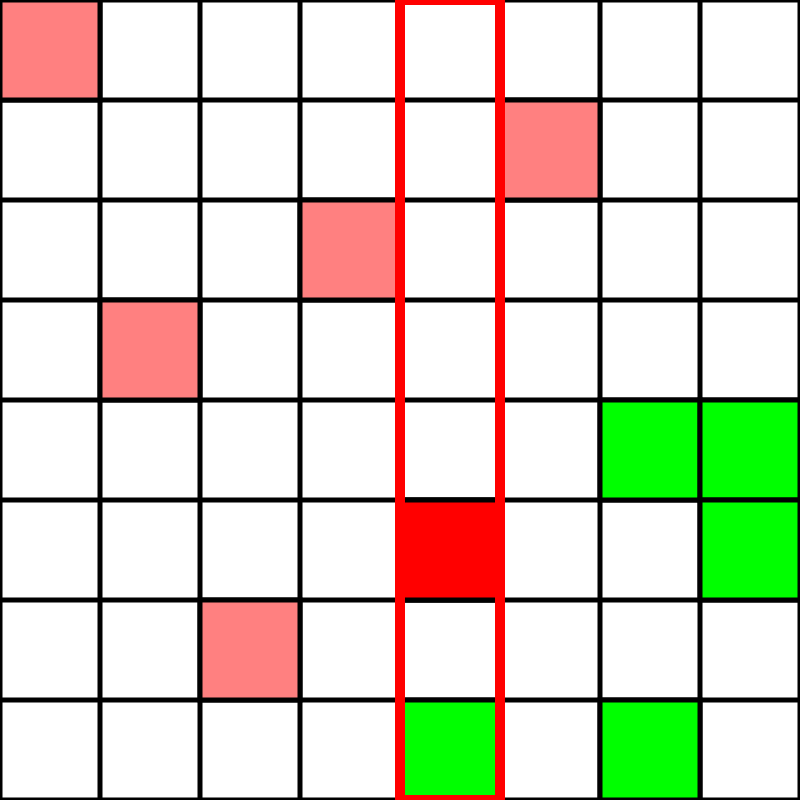
\includegraphics[width=6cm]{../sudoku/FC/frame24}
}
\end{frame}

\begin{figure}[ht]
\caption{\label{sudoku:propagationfc}Propagation Steps (Forward Checking)}
\begin{center}
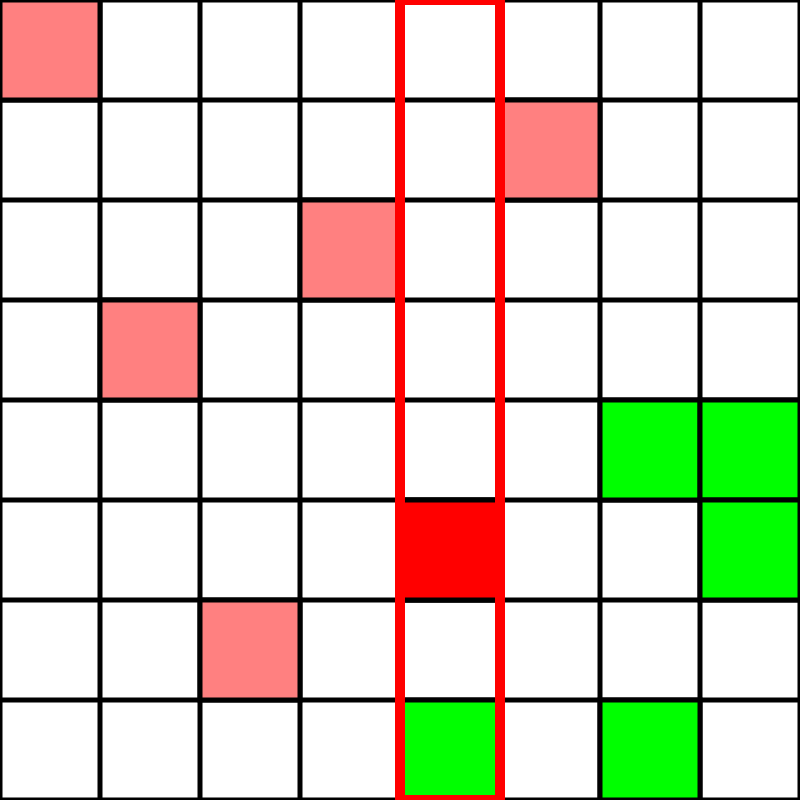
\includegraphics[width=6cm]{../sudoku/FC/frame24}
\end{center}
\end{figure}

\begin{frame}<presentation>
\frametitle{After Setup (Forward Checking)}
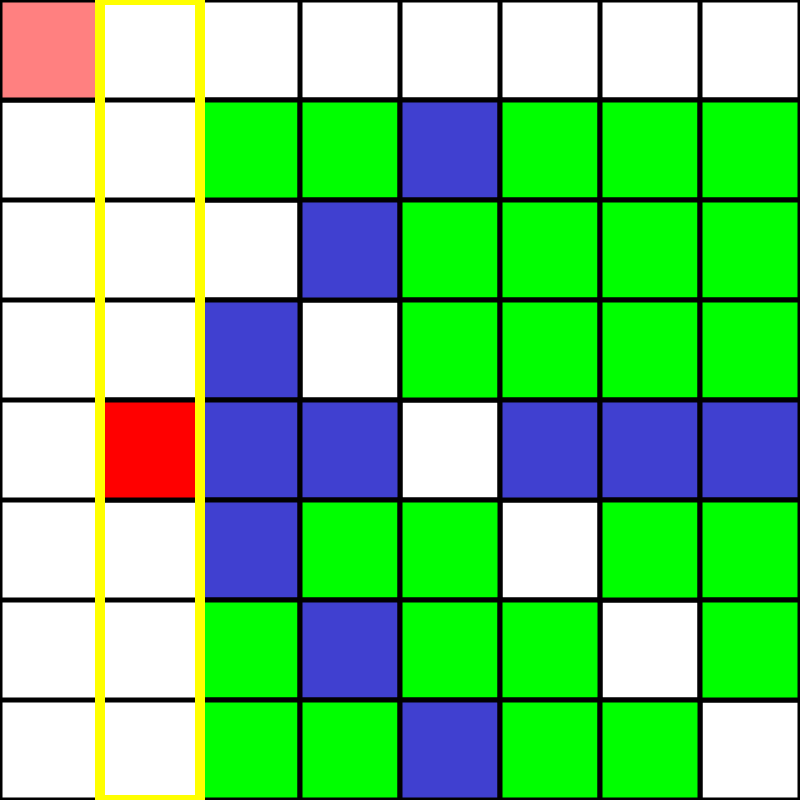
\includegraphics[width=6cm]{../sudoku/FC/frame29}
\end{frame}

\begin{figure}[ht]
\caption{\label{sudoku:aftersetupfc}After Setup (Forward Checking)}
\begin{center}
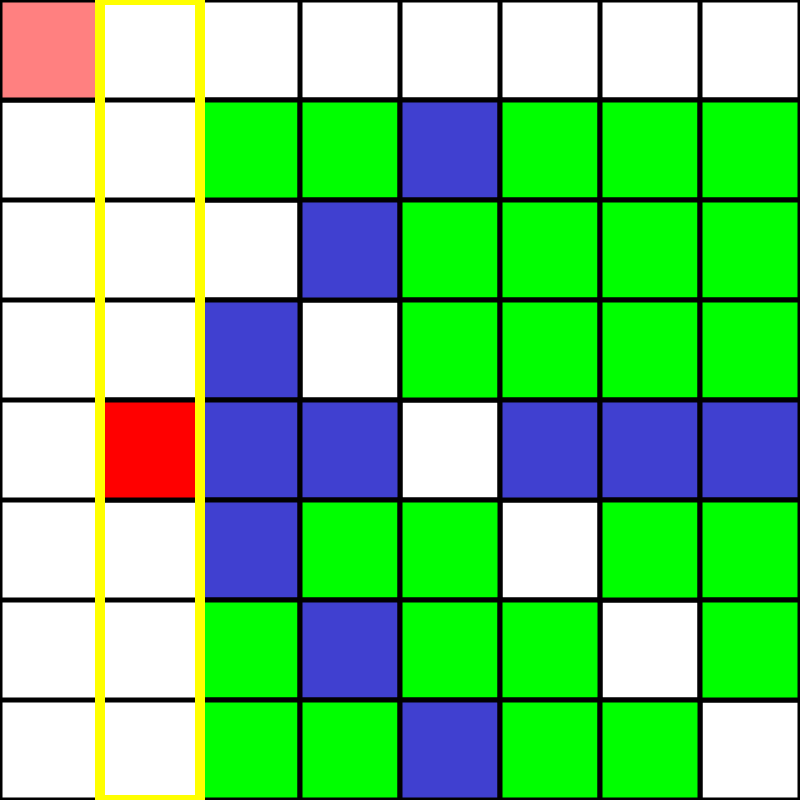
\includegraphics[width=6cm]{../sudoku/FC/frame29}
\end{center}
\end{figure}

\clearpage
\section{Improved Reasoning}

\begin{frame}
\frametitle{Can we do better?}
\begin{itemize}
\item The alldifferent constraint is missing propagation
\begin{itemize}
\item How can we do more propagation?
\item Do we know when we derive all possible information from the constraint?
\end{itemize}
\item Constraints only interact by changing domains of variables
\end{itemize}
\end{frame}

\subsection{Bounds Consistency}

\begin{frame}[fragile]
\frametitle{A Simpler Example}
\begin{semiverbatim}
include "alldifferent.mzn";

var 1..2:X;
var 1..2:Y;
var 1..3:Z;

constraint alldifferent([X,Y,Z]);

solve satisfy;
\end{semiverbatim}
\end{frame}

\begin{frame}
\frametitle{Using Forward Checking}
\begin{itemize}
\item No variable is assigned
\item No reduction of domains
\item But, values 1 and 2 can be removed from Z
\item This means that Z is assigned to 3
\end{itemize}
\end{frame}

\begin{frame}
\frametitle{Visualization of alldifferent as Graph}
\only<presentation>{
\begin{textblock}{5.5}(12,-2)
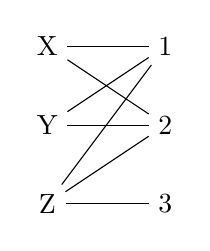
\begin{tikzpicture}
\node (X) at (1,3) {X};
\node (Y) at (1,2) {Y};
\node (Z) at (1,1) {Z};
\node (1) at (2.5,3) {1};
\node (2) at (2.5,2) {2};
\node (3) at (2.5,1) {3};
\draw  (X) -- (1);
\draw  (X) -- (2);
\draw  (Y) -- (1);
\draw  (Y) -- (2);
\draw  (Z) -- (1);
\draw  (Z) -- (2);
\draw  (Z) -- (3);
\end{tikzpicture}

\end{textblock}
}
\begin{itemize}
\item Show problem as graph with two types of nodes
\begin{itemize}
\item Variables on the left
\item Values on the right
\end{itemize}
\item If value is in domain of variable, show link between them
\item This is called a {\em bipartite} graph
\end{itemize}
\end{frame}

\begin{figure}[ht]
\caption{Visualization of alldifferent as bipartite graph}
\begin{center}
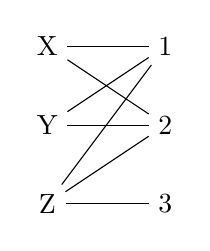
\begin{tikzpicture}
\node (X) at (1,3) {X};
\node (Y) at (1,2) {Y};
\node (Z) at (1,1) {Z};
\node (1) at (2.5,3) {1};
\node (2) at (2.5,2) {2};
\node (3) at (2.5,1) {3};
\draw  (X) -- (1);
\draw  (X) -- (2);
\draw  (Y) -- (1);
\draw  (Y) -- (2);
\draw  (Z) -- (1);
\draw  (Z) -- (2);
\draw  (Z) -- (3);
\end{tikzpicture}

\end{center}
\end{figure}

\begin{frame}[fragile]
\frametitle{A Simpler Example}
\only<presentation>{
\begin{textblock}{8}(6,0)
\only<1| handout:1>{
Value Graph for 
\begin{semiverbatim}
var 1..2:X;
\end{semiverbatim}
\begin{semiverbatim}
var 1..2:Y;
\end{semiverbatim}
\begin{semiverbatim}
var 1..3:Z;
\end{semiverbatim}
}
\only<2| handout:2>{Check interval [1,2]}
\only<3| handout:3>{\begin{itemize}
\item Find variables completely contained in interval
\item There are two: X and Y
\item This uses up the capacity of the interval
\end{itemize}
}
\only<4| handout:4>{No other variable can use that interval}
\only<5| handout:5>{Only one value left in domain of Z, this can be assigned}
\end{textblock}
\begin{tikzpicture}
\only<1| handout:1>{
\node (X) at (1,3) {X};
\node (Y) at (1,2) {Y};
\node (Z) at (1,1) {Z};
\node (1) at (3,3) {1};
\node (2) at (3,2) {2};
\node (3) at (3,1) {3};
\draw  (X) -- (1);
\draw  (X) -- (2);
\draw  (Y) -- (1);
\draw  (Y) -- (2);
\draw  (Z) -- (1);
\draw  (Z) -- (2);
\draw  (Z) -- (3);

}
\only<2| handout:2>{
\node (X) at (1,3) {X};
\node (Y) at (1,2) {Y};
\node (Z) at (1,1) {Z};
\node (1) at (3,3) [insight-blue]{1};
\node (2) at (3,2) [insight-blue]{2};
\node (3) at (3,1) {3};
\draw  (X) -- (1);
\draw  (X) -- (2);
\draw  (Y) -- (1);
\draw  (Y) -- (2);
\draw  (Z) -- (1);
\draw  (Z) -- (2);
\draw  (Z) -- (3);

}
\only<3| handout:3>{
\node (X) at (1,3) [insight-blue]{X};
\node (Y) at (1,2) [insight-blue]{Y};
\node (Z) at (1,1) {Z};
\node (1) at (3,3) [insight-blue]{1};
\node (2) at (3,2) [insight-blue]{2};
\node (3) at (3,1) {3};
\draw [thick,insight-blue] (X) -- (1);
\draw [thick,insight-blue] (X) -- (2);
\draw [thick,insight-blue] (Y) -- (1);
\draw [thick,insight-blue] (Y) -- (2);
\draw  (Z) -- (1);
\draw  (Z) -- (2);
\draw  (Z) -- (3);

}
\only<4| handout:4>{
\node (X) at (1,3) [insight-blue]{X};
\node (Y) at (1,2) [insight-blue]{Y};
\node (Z) at (1,1) {Z};
\node (1) at (3,3) [insight-blue]{1};
\node (2) at (3,2) [insight-blue]{2};
\node (3) at (3,1) {3};
\draw [insight-blue] (X) -- (1);
\draw [insight-blue] (X) -- (2);
\draw [insight-blue] (Y) -- (1);
\draw [insight-blue] (Y) -- (2);
\draw [insight-pink,thick,dotted] (Z) -- (1);
\draw [insight-pink,thick,dotted] (Z) -- (2);
\draw  (Z) -- (3);

}
\only<5| handout:5>{
\node (X) at (1,3) [insight-blue]{X};
\node (Y) at (1,2) [insight-blue]{Y};
\node (Z) at (1,1) {Z};
\node (1) at (3,3) [insight-blue]{1};
\node (2) at (3,2) [insight-blue]{2};
\node (3) at (3,1) {3};
\draw [insight-blue] (X) -- (1);
\draw [insight-blue] (X) -- (2);
\draw [insight-blue] (Y) -- (1);
\draw [insight-blue] (Y) -- (2);
\draw [insight-pink,thick] (Z) -- (3);

}
\end{tikzpicture}
}
\end{frame}


\begin{figure}[ht]
\caption{A Simpler Example}
\begin{center}
\begin{tabular}{ccccc}
a & b & c & d & e\\
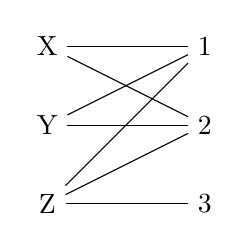
\begin{tikzpicture}\node (X) at (1,3) {X};
\node (Y) at (1,2) {Y};
\node (Z) at (1,1) {Z};
\node (1) at (3,3) {1};
\node (2) at (3,2) {2};
\node (3) at (3,1) {3};
\draw  (X) -- (1);
\draw  (X) -- (2);
\draw  (Y) -- (1);
\draw  (Y) -- (2);
\draw  (Z) -- (1);
\draw  (Z) -- (2);
\draw  (Z) -- (3);
\end{tikzpicture}
&
\begin{tikzpicture}\node (X) at (1,3) {X};
\node (Y) at (1,2) {Y};
\node (Z) at (1,1) {Z};
\node (1) at (3,3) [insight-blue]{1};
\node (2) at (3,2) [insight-blue]{2};
\node (3) at (3,1) {3};
\draw  (X) -- (1);
\draw  (X) -- (2);
\draw  (Y) -- (1);
\draw  (Y) -- (2);
\draw  (Z) -- (1);
\draw  (Z) -- (2);
\draw  (Z) -- (3);
\end{tikzpicture}
&
\begin{tikzpicture}\node (X) at (1,3) [insight-blue]{X};
\node (Y) at (1,2) [insight-blue]{Y};
\node (Z) at (1,1) {Z};
\node (1) at (3,3) [insight-blue]{1};
\node (2) at (3,2) [insight-blue]{2};
\node (3) at (3,1) {3};
\draw [thick,insight-blue] (X) -- (1);
\draw [thick,insight-blue] (X) -- (2);
\draw [thick,insight-blue] (Y) -- (1);
\draw [thick,insight-blue] (Y) -- (2);
\draw  (Z) -- (1);
\draw  (Z) -- (2);
\draw  (Z) -- (3);
\end{tikzpicture}
&
\begin{tikzpicture}\node (X) at (1,3) [insight-blue]{X};
\node (Y) at (1,2) [insight-blue]{Y};
\node (Z) at (1,1) {Z};
\node (1) at (3,3) [insight-blue]{1};
\node (2) at (3,2) [insight-blue]{2};
\node (3) at (3,1) {3};
\draw [insight-blue] (X) -- (1);
\draw [insight-blue] (X) -- (2);
\draw [insight-blue] (Y) -- (1);
\draw [insight-blue] (Y) -- (2);
\draw [insight-pink,thick,dotted] (Z) -- (1);
\draw [insight-pink,thick,dotted] (Z) -- (2);
\draw  (Z) -- (3);
\end{tikzpicture}
&
\begin{tikzpicture}\node (X) at (1,3) [insight-blue]{X};
\node (Y) at (1,2) [insight-blue]{Y};
\node (Z) at (1,1) {Z};
\node (1) at (3,3) [insight-blue]{1};
\node (2) at (3,2) [insight-blue]{2};
\node (3) at (3,1) {3};
\draw [insight-blue] (X) -- (1);
\draw [insight-blue] (X) -- (2);
\draw [insight-blue] (Y) -- (1);
\draw [insight-blue] (Y) -- (2);
\draw [insight-pink,thick] (Z) -- (3);
\end{tikzpicture}
\end{tabular}
\end{center}
\end{figure}

%\caption{Value Graph for X :: 1..2, Y :: 1..2, Z :: 1..3}
%\caption{Check interval [1,2]}
%\caption{Find variables completely contained in interval}
%\caption{No other variable can use that interval}
%\caption{Only one value left in domain of Z, this can be assigned}


\begin{frame}
\frametitle{Idea (Hall Intervals)}
\begin{itemize}
\item Take each interval of possible values, say size $N$
\item Find all $K$ variables whose domain is completely contained in interval
\item If $K>N$ then the constraint is infeasible
\item If $K=N$ then no other variable can use that interval
\item Remove values from such variables if their bounds change
\item If $K<N$ do nothing
\item Re-check whenever domain bounds change
\end{itemize}
\end{frame}

\begin{frame}
\frametitle{Implementation}
\begin{itemize}
\item Problem: Too many intervals ($O(n^2)$) to consider
\item Solution:
\begin{itemize}
\item Check only those intervals which update bounds
\item Enumerate intervals incrementally
\item Starting from lowest(highest) value
\item Using sorted list of variables
\end{itemize}
\item Complexity: $O(n\log(n))$ in standard implementations
\item Important: Only looks at min/max bounds of variables
\end{itemize}
\end{frame}

\begin{frame}
\frametitle{Bounds Consistency}
\begin{block}{Definition}
A constraint achieves {\em bounds consistency}, if for the lower and upper bound of every variable, it is possible to find values for all other variables between their lower and upper bounds which satisfy the constraint.
\end{block}
\end{frame}

\begin{frame}[fragile]
\frametitle{Annotation: :: bounds}
\begin{semiverbatim}
include "alldifferent.mzn";

var 1..2:X;
var 1..2:Y;
var 1..3:Z;

constraint alldifferent([X,Y,Z]) :: bounds;
solve satisfy;
\end{semiverbatim}
\end{frame}

\begin{frame}
  \frametitle{Running with Gecode Gist}
  \begin{tabular}{cc}
    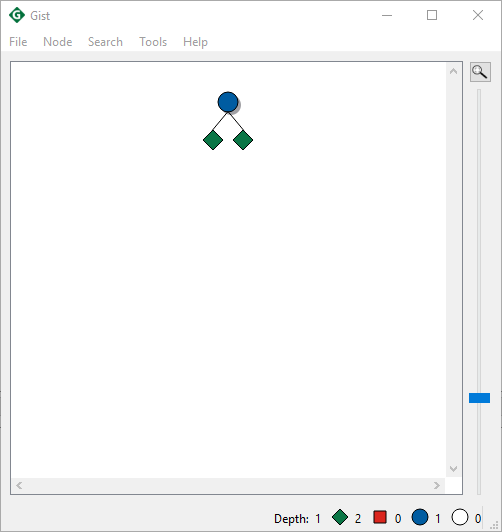
\includegraphics[width=5cm]{../sudoku/images/xyzgist}
    &
    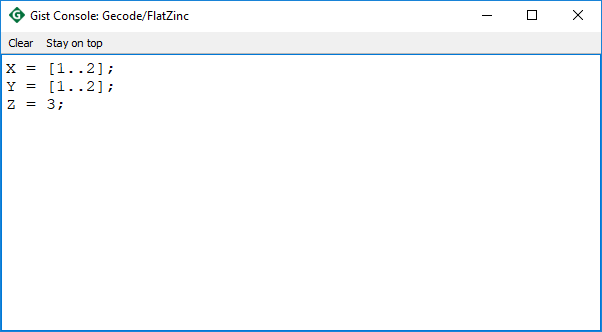
\includegraphics[width=5cm]{../sudoku/images/xyzgistinspector}
    \\
    All Solutions & Node Inspector (Root)
  \end{tabular}
\end{frame}


\begin{frame}
\frametitle{Can we do even better?}
\begin{itemize}
\item Bounds consistency only considers min/max bounds
\item Ignores ``holes'' in domain
\item Sometimes we can improve propagation looking at those holes
\end{itemize}
\end{frame}

\begin{frame}[fragile]
\frametitle{Another Simple Example}
\begin{semiverbatim}
include "alldifferent.mzn";

var \{1,3\}:X; % note enumerated domain
var \{1,3\}:Y;
var 1..3:Z; % note domain as interval

% annotated constraint
constraint alldifferent([X,Y,Z]) :: bounds;
solve satisfy;
\end{semiverbatim}
\end{frame}

\begin{frame}<presentation>[fragile]
\frametitle{Another Simple Example}
\only<presentation>{
\begin{textblock}{8}(6,0)
\only<1| handout:1>{Value Graph for 
  \begin{semiverbatim}
var \{1,3\}:X;
\end{semiverbatim}
\begin{semiverbatim}
var \{1,3\}:Y;
\end{semiverbatim}
\begin{semiverbatim}
var 1..3:Z;
\end{semiverbatim}
}
\only<2| handout:2>{\begin{itemize}
\item Check interval [1,2]
\item No domain of a variable completely contained in interval
\item No propagation
\end{itemize}}
\only<3| handout:3>{\begin{itemize}
\item Check interval [2,3]
\item No domain of a variable completely contained in interval
\item No propagation
\end{itemize}}
\only<4| handout:4>{But, more propagation is possible, there are only two solutions}
\only<5| handout:5>{Solution 1: assignment in blue}
\only<6| handout:6>{Solution 2: assignment in green}
\end{textblock}
\begin{tikzpicture}
\only<1| handout:1>{
\node (X) at (1,3) {X};
\node (Y) at (1,2) {Y};
\node (Z) at (1,1) {Z};
\node (1) at (3,3) {1};
\node (2) at (3,2) {2};
\node (3) at (3,1) {3};
\draw  (X) -- (1);
\draw  (X) -- (3);
\draw  (Y) -- (1);
\draw  (Y) -- (3);
\draw  (Z) -- (1);
\draw  (Z) -- (2);
\draw  (Z) -- (3);

}
\only<2| handout:2>{
\node (X) at (1,3) {X};
\node (Y) at (1,2) {Y};
\node (Z) at (1,1) {Z};
\node (1) at (3,3) [insight-blue] {1};
\node (2) at (3,2) [insight-blue] {2};
\node (3) at (3,1) {3};
\draw  (X) -- (1);
\draw  (X) -- (3);
\draw  (Y) -- (1);
\draw  (Y) -- (3);
\draw  (Z) -- (1);
\draw  (Z) -- (2);
\draw  (Z) -- (3);

}
\only<3| handout:3>{
\node (X) at (1,3) {X};
\node (Y) at (1,2) {Y};
\node (Z) at (1,1) {Z};
\node (1) at (3,3) {1};
\node (2) at (3,2) [insight-blue] {2};
\node (3) at (3,1) [insight-blue] {3};
\draw  (X) -- (1);
\draw  (X) -- (3);
\draw  (Y) -- (1);
\draw  (Y) -- (3);
\draw  (Z) -- (1);
\draw  (Z) -- (2);
\draw  (Z) -- (3);

}
\only<4| handout:4>{
\node (X) at (1,3) {X};
\node (Y) at (1,2) {Y};
\node (Z) at (1,1) {Z};
\node (1) at (3,3) {1};
\node (2) at (3,2) {2};
\node (3) at (3,1) {3};
\draw  (X) -- (1);
\draw  (X) -- (3);
\draw  (Y) -- (1);
\draw  (Y) -- (3);
\draw  (Z) -- (1);
\draw  (Z) -- (2);
\draw  (Z) -- (3);

}
\only<5| handout:5>{
\node (X) at (1,3) {X};
\node (Y) at (1,2) {Y};
\node (Z) at (1,1) {Z};
\node (1) at (3,3) {1};
\node (2) at (3,2) {2};
\node (3) at (3,1) {3};
\draw [insight-blue,thick] (X) -- (1);
\draw [dotted] (X) -- (3);
\draw [dotted] (Y) -- (1);
\draw [insight-blue,thick] (Y) -- (3);
\draw [dotted] (Z) -- (1);
\draw [insight-blue,thick] (Z) -- (2);
\draw [dotted] (Z) -- (3);

}
\only<6| handout:6>{
\node (X) at (1,3) {X};
\node (Y) at (1,2) {Y};
\node (Z) at (1,1) {Z};
\node (1) at (3,3) {1};
\node (2) at (3,2) {2};
\node (3) at (3,1) {3};
\draw [dotted] (X) -- (1);
\draw [green,thick] (X) -- (3);
\draw [green,thick] (Y) -- (1);
\draw [dotted] (Y) -- (3);
\draw [dotted] (Z) -- (1);
\draw [green,thick] (Z) -- (2);
\draw [dotted] (Z) -- (3);

}
\end{tikzpicture}
\only<7| handout:7>{
\begin{center}
\begin{tabular}{ccc}
Solution 1 & Solution 2 & Combined \\
\begin{tikzpicture}
\node (X) at (1,3) {X};
\node (Y) at (1,2) {Y};
\node (Z) at (1,1) {Z};
\node (1) at (3,3) {1};
\node (2) at (3,2) {2};
\node (3) at (3,1) {3};
\draw [insight-blue,thick] (X) -- (1);
\draw [dotted] (X) -- (3);
\draw [dotted] (Y) -- (1);
\draw [insight-blue,thick] (Y) -- (3);
\draw [dotted] (Z) -- (1);
\draw [insight-blue,thick] (Z) -- (2);
\draw [dotted] (Z) -- (3);

\end{tikzpicture}
&
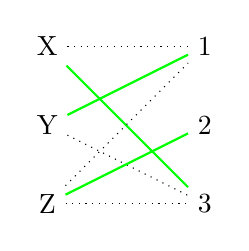
\begin{tikzpicture}
\node (X) at (1,3) {X};
\node (Y) at (1,2) {Y};
\node (Z) at (1,1) {Z};
\node (1) at (3,3) {1};
\node (2) at (3,2) {2};
\node (3) at (3,1) {3};
\draw [dotted] (X) -- (1);
\draw [green,thick] (X) -- (3);
\draw [green,thick] (Y) -- (1);
\draw [dotted] (Y) -- (3);
\draw [dotted] (Z) -- (1);
\draw [green,thick] (Z) -- (2);
\draw [dotted] (Z) -- (3);

\end{tikzpicture}
&
\begin{tikzpicture}
\node (X) at (1,3) {X};
\node (Y) at (1,2) {Y};
\node (Z) at (1,1) {Z};
\node (1) at (3,3) {1};
\node (2) at (3,2) {2};
\node (3) at (3,1) {3};
\draw [insight-blue] (X) -- (1);
\draw [insight-green] (X) -- (3);
\draw [insight-green] (Y) -- (1);
\draw [insight-blue] (Y) -- (3);
\draw [insight-pink,thick,dotted] (Z) -- (1);
\draw [insight-green] (Z) -- (2);
\draw [insight-pink,thick,dotted] (Z) -- (3);

\end{tikzpicture}
\end{tabular}
\end{center}

}
\begin{textblock}{9}(2,0)
\only<7| handout:7>{Combining solutions shows that Z=1 and Z=3 are not possible.}
\only<8| handout:7>{Can we deduce this without enumerating solutions?}
\end{textblock}
}
\end{frame}

\begin{frame}
  \frametitle{Bounds Consistency with Gecode Gist: No Propagation}
  \begin{tabular}{cc}
    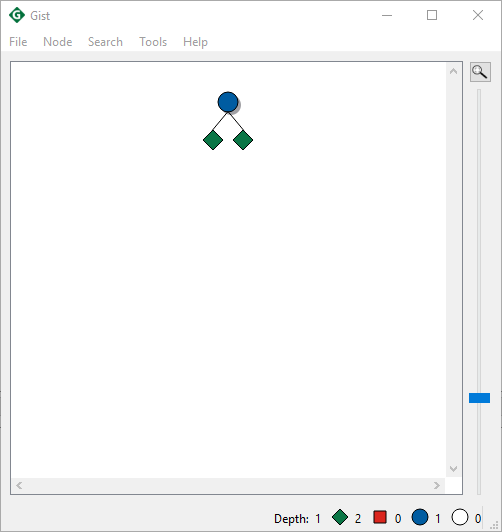
\includegraphics[width=5cm]{../sudoku/images/xyzgistmissing}
    &
    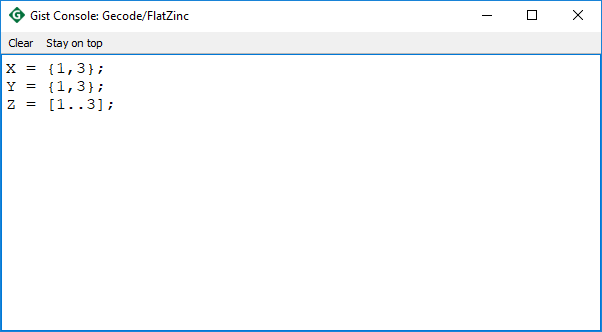
\includegraphics[width=5cm]{../sudoku/images/xyzgistmissinginspector}
    \\
    All Solutions & Node Inspector (Root)
  \end{tabular}
\end{frame}

%\caption{Value Graph for X :: [1,3], Y :: [1,3], Z :: 1..3}
%\caption{Check interval [1,2], no propagation}
%\caption{Check interval [2,3], no propagation}
%\caption{But, more propagation is possible, there are only two solutions}
%\caption{Solution 1: assignment in blue}
%\caption{Solution 2: assignment in green}
%\caption{Combining solutions shows that Z=1 and Z=3 are not possible. Can we deduce this without enumerating solutions?}

\begin{figure}[ht]
\caption{Another Example}
\begin{center}
\begin{tabular}{ccc}
a & b & c \\
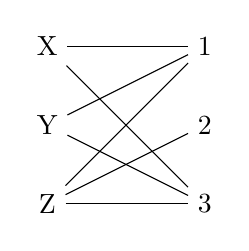
\begin{tikzpicture}\node (X) at (1,3) {X};
\node (Y) at (1,2) {Y};
\node (Z) at (1,1) {Z};
\node (1) at (3,3) {1};
\node (2) at (3,2) {2};
\node (3) at (3,1) {3};
\draw  (X) -- (1);
\draw  (X) -- (3);
\draw  (Y) -- (1);
\draw  (Y) -- (3);
\draw  (Z) -- (1);
\draw  (Z) -- (2);
\draw  (Z) -- (3);
\end{tikzpicture}
&
\begin{tikzpicture}\node (X) at (1,3) {X};
\node (Y) at (1,2) {Y};
\node (Z) at (1,1) {Z};
\node (1) at (3,3) [insight-blue] {1};
\node (2) at (3,2) [insight-blue] {2};
\node (3) at (3,1) {3};
\draw  (X) -- (1);
\draw  (X) -- (3);
\draw  (Y) -- (1);
\draw  (Y) -- (3);
\draw  (Z) -- (1);
\draw  (Z) -- (2);
\draw  (Z) -- (3);
\end{tikzpicture}
&
\begin{tikzpicture}\node (X) at (1,3) {X};
\node (Y) at (1,2) {Y};
\node (Z) at (1,1) {Z};
\node (1) at (3,3) {1};
\node (2) at (3,2) [insight-blue] {2};
\node (3) at (3,1) [insight-blue] {3};
\draw  (X) -- (1);
\draw  (X) -- (3);
\draw  (Y) -- (1);
\draw  (Y) -- (3);
\draw  (Z) -- (1);
\draw  (Z) -- (2);
\draw  (Z) -- (3);
\end{tikzpicture}
\end{tabular}
\end{center}
\end{figure}

\begin{figure}[ht]
\caption{Another Example (Continued)}
\begin{center}
\begin{tabular}{ccc}
d & e & f \\
\begin{tikzpicture}\node (X) at (1,3) {X};
\node (Y) at (1,2) {Y};
\node (Z) at (1,1) {Z};
\node (1) at (3,3) {1};
\node (2) at (3,2) {2};
\node (3) at (3,1) {3};
\draw [insight-blue,thick] (X) -- (1);
\draw [dotted] (X) -- (3);
\draw [dotted] (Y) -- (1);
\draw [insight-blue,thick] (Y) -- (3);
\draw [dotted] (Z) -- (1);
\draw [insight-blue,thick] (Z) -- (2);
\draw [dotted] (Z) -- (3);
\end{tikzpicture}
&
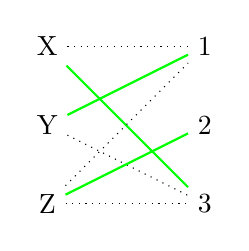
\begin{tikzpicture}\node (X) at (1,3) {X};
\node (Y) at (1,2) {Y};
\node (Z) at (1,1) {Z};
\node (1) at (3,3) {1};
\node (2) at (3,2) {2};
\node (3) at (3,1) {3};
\draw [dotted] (X) -- (1);
\draw [green,thick] (X) -- (3);
\draw [green,thick] (Y) -- (1);
\draw [dotted] (Y) -- (3);
\draw [dotted] (Z) -- (1);
\draw [green,thick] (Z) -- (2);
\draw [dotted] (Z) -- (3);
\end{tikzpicture}
&
\begin{tikzpicture}\node (X) at (1,3) {X};
\node (Y) at (1,2) {Y};
\node (Z) at (1,1) {Z};
\node (1) at (3,3) {1};
\node (2) at (3,2) {2};
\node (3) at (3,1) {3};
\draw [insight-blue] (X) -- (1);
\draw [insight-green] (X) -- (3);
\draw [insight-green] (Y) -- (1);
\draw [insight-blue] (Y) -- (3);
\draw [insight-pink,thick,dotted] (Z) -- (1);
\draw [insight-green] (Z) -- (2);
\draw [insight-pink,thick,dotted] (Z) -- (3);
\end{tikzpicture}
\end{tabular}
\end{center}
\end{figure}



\begin{frame}
\frametitle{Solutions and Maximal Matchings}
\begin{itemize}
\item A {\em Matching} is subset of edges which do not coincide in any node
\item No matching can have more edges than number of variables
\item Every solution corresponds to a {\em maximal matching} and vice versa
\item If a link does not belong to some maximal matching, then it can be removed 
\end{itemize}
\end{frame}

\begin{frame}
\frametitle{Implementation}
\begin{itemize}
\item Possible to compute all links which belong to some matching
\begin{itemize}
\item Without enumerating all of them!
\end{itemize}
\item Enough to compute {\bf one} maximal matching
\item Requires algorithm for {\em strongly connected components}
\item Extra work required if more values than variables
\item All links (values in domains) which are not supported can be removed
\item Complexity: $O(n^{1.5}d)$
\end{itemize}
\end{frame}

\begin{frame}
\frametitle{Domain Consistency}
\begin{block}{Definition}
A constraint achieves {\em domain consistency}, if for every variable and for every value in its domain, it is possible to find values in the domains of all other variables which satisfy the constraint.
\end{block}
\begin{itemize}
\item Also called {\em generalized arc consistency (GAC)}
\item or {\em hyper arc consistency}
\end{itemize}
\end{frame}

\begin{frame}[fragile]
\frametitle{Simple Example Revisited}
\begin{semiverbatim}
include "alldifferent.mzn";

var \{1,3\}:X; % note enumerated domain
var \{1,3\}:Y;
var 1..3:Z; % note domain as interval

% note different annotation
constraint alldifferent([X,Y,Z]) :: domain;
solve satisfy;
\end{semiverbatim}
\end{frame}

\begin{frame}
  \frametitle{Domain Consistency with Gecode Gist: Propagation}
  \begin{tabular}{cc}
    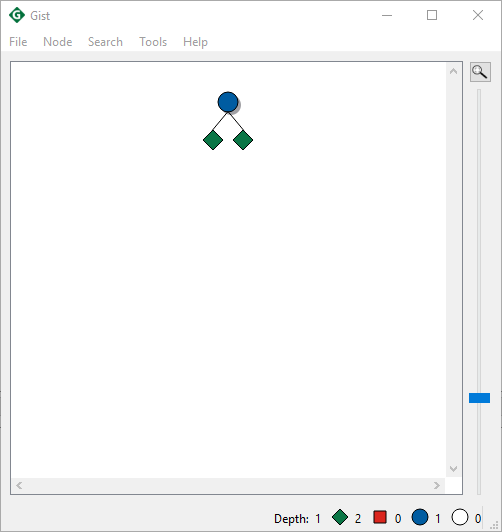
\includegraphics[width=5cm]{../sudoku/images/xyzgistdomain}
    &
    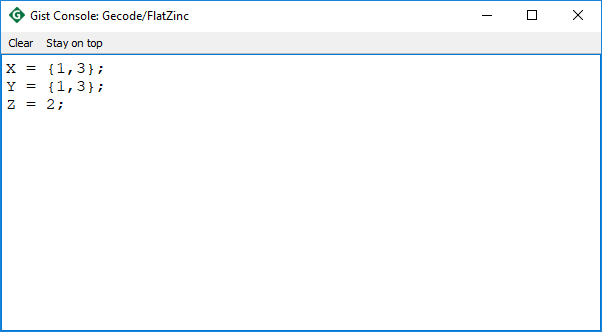
\includegraphics[width=5cm]{../sudoku/images/xyzgistdomaininspector}
    \\
    All Solutions & Node Inspector (Root)
  \end{tabular}
\end{frame}


\begin{frame}
\frametitle{Can we still do better?}
\begin{itemize}
\item NO! This extracts all information from this one constraint
\item We could perhaps improve speed, but not propagation
\item But possible to use different model
\item Or model interaction of multiple constraints
\end{itemize}
\end{frame}

\begin{frame}
\frametitle{Should all constraints achieve domain consistency?}
\begin{itemize}
\item Domain consistency is usually more expensive than bounds consistency
\begin{itemize}
\item Overkill for simple problems
\item Nice to have choices
\end{itemize}
\item For some constraints achieving domain consistency is NP-hard
\begin{itemize}
\item We have to live with more restricted propagation
\end{itemize}
\end{itemize}
\end{frame}


\subsection{Domain Consistency}

\begin{frame}[fragile]
  \frametitle{Modified MiniZinc Program}
  \label{sudoku:minizinc mod}
  \small
\begin{semiverbatim}
int: s;
int: n=s*s;
array[1..n,1..n] of var 1..n: puzzle;

include "sudoku.dzn";

include "alldifferent.mzn";

constraint forall(i in 1..n)
    (alldifferent([puzzle[i,j]| j in 1..n])::domain);
constraint forall(j in 1..n)
    (alldifferent([ puzzle[i,j]| i in 1..n])::domain);
constraint forall(i,j in 1..s)
    (alldifferent([puzzle[s*(i-1)+p, s*(j-1)+q]|
                  p,q in 1..s])::domain);

solve satisfy;
\end{semiverbatim}
\end{frame}

\begin{frame}[fragile]
\frametitle{Modified Choco-solver Sudoku Model}
\label{sudoku:choco mod}
\tiny
\begin{verbatim}
    Model model = new Model("Sudoku");
    int blockSize = 3;
    int m = blockSize*blockSize;

    IntVar[][] vars = new IntVar[m][m];
    for(int i=0;i<m;i++){
        for(int j=0;j<m;j++){
            vars[i][j] =  model.intVar("X"+i+""+j, 1, m);
            if (data[i][j]>0) {
                model.arithm(vars[i][j],"=",data[i][j]).post();
            }
        }
    }
	// Consistency level AC: domain consistency, BC: bounds consistency, default: mix
    for(int i=0;i<m;i++){
        model.allDifferent(row(i,m,vars),AC).post();
        model.allDifferent(column(i,m,vars),AC).post();
    }
    for(int i=0;i<m;i+=blockSize){
        for(int j=0;j<m;j+=blockSize){
            model.allDifferent(block(i,j,blockSize,vars),AC).post();
        }
    }
    Solver solver = model.getSolver();
    solver.solve();
\end{verbatim}
\end{frame}


\begin{frame}<presentation>
\frametitle{Initial State (Domain Consistency)}
\includegraphics[width=6cm]{../sudoku/DC/frame1}
\end{frame}

\begin{figure}[ht]
\caption{\label{sudoku:initialstatedc}Initial State (Domain Consistency)}
\begin{center}
\includegraphics[width=6cm]{../sudoku/DC/frame1}
\end{center}
\end{figure}


\begin{frame}<presentation>
\frametitle{Propagation Steps (Domain Consistency)}
\only<beamer>{
\only<1>{\includegraphics[width=6cm]{../sudoku/DC/frame1}}
\only<2>{\includegraphics[width=6cm]{../sudoku/DC/frame2}}
\only<3>{\includegraphics[width=6cm]{../sudoku/DC/frame3}}
\only<4>{\includegraphics[width=6cm]{../sudoku/DC/frame4}}
\only<5>{\includegraphics[width=6cm]{../sudoku/DC/frame5}}
\only<6>{\includegraphics[width=6cm]{../sudoku/DC/frame6}}
\only<7>{\includegraphics[width=6cm]{../sudoku/DC/frame7}}
\only<8>{\includegraphics[width=6cm]{../sudoku/DC/frame8}}
\only<9>{\includegraphics[width=6cm]{../sudoku/DC/frame9}}
\only<10>{\includegraphics[width=6cm]{../sudoku/DC/frame10}}
\only<11>{\includegraphics[width=6cm]{../sudoku/DC/frame11}}
\only<12>{\includegraphics[width=6cm]{../sudoku/DC/frame12}}
\only<13>{\includegraphics[width=6cm]{../sudoku/DC/frame13}}
\only<14>{\includegraphics[width=6cm]{../sudoku/DC/frame14}}
\only<15>{\includegraphics[width=6cm]{../sudoku/DC/frame15}}
\only<16>{\includegraphics[width=6cm]{../sudoku/DC/frame16}}
\only<17>{\includegraphics[width=6cm]{../sudoku/DC/frame17}}
\only<18>{\includegraphics[width=6cm]{../sudoku/DC/frame18}}
\only<19>{\includegraphics[width=6cm]{../sudoku/DC/frame19}}
\only<20>{\includegraphics[width=6cm]{../sudoku/DC/frame20}}
\only<21>{\includegraphics[width=6cm]{../sudoku/DC/frame21}}
\only<22>{\includegraphics[width=6cm]{../sudoku/DC/frame22}}
\only<23>{\includegraphics[width=6cm]{../sudoku/DC/frame23}}
\only<24>{\includegraphics[width=6cm]{../sudoku/DC/frame24}}
\only<25>{\includegraphics[width=6cm]{../sudoku/DC/frame25}}
\only<26>{\includegraphics[width=6cm]{../sudoku/DC/frame26}}
\only<27>{\includegraphics[width=6cm]{../sudoku/DC/frame27}}
\only<28>{\includegraphics[width=6cm]{../sudoku/DC/frame28}}
\only<29>{\includegraphics[width=6cm]{../sudoku/DC/frame29}}
\vfill
\hyperlinkframestart<2-29>{\beamerreturnbutton{Back to Start}}
\hyperlinkframeend<1-28>{\beamerskipbutton{Skip Animation}}
}
\only<handout>{
\includegraphics[width=6cm]{../sudoku/DC/frame24}
}
\end{frame}

\begin{figure}[ht]
\caption{\label{sudoku:propagationdc}Propagation Steps (Domain Consistency)}
\begin{center}
\includegraphics[width=6cm]{../sudoku/DC/frame24}
\end{center}
\end{figure}


\begin{frame}<presentation>
\frametitle{After Setup (Domain Consistency)}
\includegraphics[width=6cm]{../sudoku/DC/frame29}
\end{frame}

\begin{figure}[ht]
\caption{\label{sudoku:aftersetupdc}After Setup (Domain Consistency)}
\begin{center}
\includegraphics[width=6cm]{../sudoku/DC/frame29}
\end{center}
\end{figure}


\subsection{Comparison}

\begin{frame}<presentation>
\frametitle{Comparison}
\begin{tabular}{ccc}
Forward Checking & Bounds Consistency & Domain Consistency \\
\includegraphics[width=3cm]{../sudoku/FC/frame29}
&
\includegraphics[width=3cm]{../sudoku/BC/frame29}
&
\includegraphics[width=3cm]{../sudoku/DC/frame29}
\end{tabular}
\end{frame}

\begin{figure}[ht]
\caption{\label{sudoku:comparison}Comparison}
\begin{center}
\begin{tabular}{ccc}
Forward Checking & Bounds Consistency & Domain Consistency \\
\includegraphics[width=4cm]{../sudoku/FC/frame29}
&
\includegraphics[width=4cm]{../sudoku/BC/frame29}
&
\includegraphics[width=4cm]{../sudoku/DC/frame29}
\end{tabular}
\end{center}
\end{figure}

\begin{frame}
\frametitle{Typical?}
\begin{itemize}
\item This does not always happen
\item Sometimes, two methods produce same amount of propagation
\item Possible to predict in certain special cases
\item In general, tradeoff between speed and propagation
\item Not always fastest to remove inconsistent values early
\item But often required to find a solution at all
\end{itemize}
\end{frame}

\clearpage
\section{Search}

\begin{frame}
\frametitle{Simple search routine}
\begin{itemize}
\item Enumerate variables in given order
\item Try values starting from smallest one in domain
\item Complete, chronological backtracking
\item Advantage: Results can be compared with each other
\item Disadvantage: Usually not a very good strategy
\end{itemize}
\end{frame}

\begin{frame}[fragile]
  \frametitle{Asking for Naive Search in MiniZinc}
  \begin{semiverbatim}
    solve :: int\_search(
      puzzle,    
      input\_order,   
      indomain\_min)    
    satisfy;
  \end{semiverbatim}
\end{frame}

\begin{frame}<presentation>[label=searchfc]
\frametitle{Search Tree (Forward Checking)}
\only<beamer>{
\begin{textblock}{5.5}(9.5,0)
\only<1>{\includegraphics[width=4cm]{../sudoku/FC/frame29}}
\only<2>{\includegraphics[width=4cm]{../sudoku/FC/frame30}}
\only<3>{\includegraphics[width=4cm]{../sudoku/FC/frame31}}
\only<4>{\includegraphics[width=4cm]{../sudoku/FC/frame32}}
\only<5>{\includegraphics[width=4cm]{../sudoku/FC/frame33}}
\only<6>{\includegraphics[width=4cm]{../sudoku/FC/frame34}}
\only<7>{\includegraphics[width=4cm]{../sudoku/FC/frame35}}
\only<8>{\includegraphics[width=4cm]{../sudoku/FC/frame36}}
\only<9>{\includegraphics[width=4cm]{../sudoku/FC/frame37}}
\only<10>{\includegraphics[width=4cm]{../sudoku/FC/frame38}}
\only<11>{\includegraphics[width=4cm]{../sudoku/FC/frame39}}
\only<12>{\includegraphics[width=4cm]{../sudoku/FC/frame40}}
\only<13>{\includegraphics[width=4cm]{../sudoku/FC/frame41}}
\only<14>{\includegraphics[width=4cm]{../sudoku/FC/frame42}}
\only<15>{\includegraphics[width=4cm]{../sudoku/FC/frame43}}
\only<16>{\includegraphics[width=4cm]{../sudoku/FC/frame44}}
\only<17>{\includegraphics[width=4cm]{../sudoku/FC/frame45}}
\only<18>{\includegraphics[width=4cm]{../sudoku/FC/frame46}}
\only<19>{\includegraphics[width=4cm]{../sudoku/FC/frame47}}
\only<20>{\includegraphics[width=4cm]{../sudoku/FC/frame48}}
\end{textblock}
\only<1>{\includegraphics[width=8cm]{../sudoku/FC/tree_expanded_1}}
\only<2>{\includegraphics[width=8cm]{../sudoku/FC/tree_expanded_2}}
\only<3>{\includegraphics[width=8cm]{../sudoku/FC/tree_expanded_3}}
\only<4>{\includegraphics[width=8cm]{../sudoku/FC/tree_expanded_4}}
\only<5>{\includegraphics[width=8cm]{../sudoku/FC/tree_expanded_5}}
\only<6>{\includegraphics[width=8cm]{../sudoku/FC/tree_expanded_6}}
\only<7>{\includegraphics[width=8cm]{../sudoku/FC/tree_expanded_7}}
\only<8>{\includegraphics[width=8cm]{../sudoku/FC/tree_expanded_8}}
\only<9>{\includegraphics[width=8cm]{../sudoku/FC/tree_expanded_9}}
\only<10>{\includegraphics[width=8cm]{../sudoku/FC/tree_expanded_10}}
\only<11>{\includegraphics[width=8cm]{../sudoku/FC/tree_expanded_11}}
\only<12>{\includegraphics[width=8cm]{../sudoku/FC/tree_expanded_12}}
\only<13>{\includegraphics[width=8cm]{../sudoku/FC/tree_expanded_13}}
\only<14>{\includegraphics[width=8cm]{../sudoku/FC/tree_expanded_14}}
\only<15>{\includegraphics[width=8cm]{../sudoku/FC/tree_expanded_15}}
\only<16>{\includegraphics[width=8cm]{../sudoku/FC/tree_expanded_16}}
\only<17>{\includegraphics[width=8cm]{../sudoku/FC/tree_expanded_17}}
\only<18>{\includegraphics[width=8cm]{../sudoku/FC/tree_expanded_18}}
\only<19>{\includegraphics[width=8cm]{../sudoku/FC/tree_expanded_19}}
\only<20>{\includegraphics[width=8cm]{../sudoku/FC/tree_expanded_20}}
\vfill
\hyperlinkframestart<2-20>{\beamerreturnbutton{Back to Start}}
\hyperlinkframeend<1-19>{\beamerskipbutton{Skip Animation}}
}
\only<handout>{
\includegraphics[width=8cm]{../sudoku/FC/tree_expanded_20}
}
\end{frame}

\begin{figure}[ht]
\caption{\label{sudoku:searchtreefc}Search Tree (Forward Checking)}
\begin{center}
\includegraphics[width=12cm]{../sudoku/FC/tree_expanded_20}
\end{center}
\end{figure}



\begin{frame}<presentation>[label=seachbc]
\frametitle{Search Tree (Bounds Consistency)}
\only<beamer>{
\begin{textblock}{5.5}(9,0)
\only<1>{\includegraphics[width=4cm]{../sudoku/BC/frame29}}
\only<2>{\includegraphics[width=4cm]{../sudoku/BC/frame30}}
\only<3>{\includegraphics[width=4cm]{../sudoku/BC/frame31}}
\only<4>{\includegraphics[width=4cm]{../sudoku/BC/frame32}}
\end{textblock}
\only<1>{\includegraphics[width=8cm]{../sudoku/BC/tree_expanded_1}}
\only<2>{\includegraphics[width=8cm]{../sudoku/BC/tree_expanded_2}}
\only<3>{\includegraphics[width=8cm]{../sudoku/BC/tree_expanded_3}}
\only<4>{\includegraphics[width=8cm]{../sudoku/BC/tree_expanded_4}}
\vfill
\hyperlinkframestart<2-4>{\beamerreturnbutton{Back to Start}}
\hyperlinkframeend<1-3>{\beamerskipbutton{Skip Animation}}
}
\only<handout>{
\includegraphics[width=8cm]{../sudoku/BC/tree_expanded_4}
}
\end{frame}

\begin{figure}[ht]
\caption{\label{sudoku:searchtreebc}Search Tree (Bounds Consistency)}
\begin{center}
\includegraphics[width=10cm]{../sudoku/BC/tree_expanded_4}
\end{center}
\end{figure}


\begin{frame}<presentation>[label=searchgac]
\frametitle{Search Tree (Domain Consistency)}
\only<beamer>{
\begin{textblock}{5.5}(9,0)
\only<1>{\includegraphics[width=4cm]{../sudoku/DC/frame29}}
\only<2>{\includegraphics[width=4cm]{../sudoku/DC/frame30}}
\end{textblock}
\only<1>{\includegraphics[width=8cm]{../sudoku/DC/tree_expanded_1}}
\only<2>{\includegraphics[width=8cm]{../sudoku/DC/tree_expanded_2}}
\vfill
\hyperlinkframestart<2>{\beamerreturnbutton{Back to Start}}
\hyperlinkframeend<1>{\beamerskipbutton{Skip Animation}}
}
\only<handout>{
\includegraphics[width=8cm]{../sudoku/DC/tree_expanded_2}
}
\end{frame}

\begin{figure}[ht]
\caption{\label{sudoku:searchtreedc}Search Tree (Domain Consistency)}
\begin{center}
\includegraphics[width=10cm]{../sudoku/DC/tree_expanded_2}
\end{center}
\end{figure}

\begin{frame}
  \frametitle{Trading Propagation Against Search}
  \begin{itemize}
  \item If we perform more propagation, search is more constrained
  \item Fewer values left, fewer alternatives to explore in search
  \item Best compromise is not obvious
  \item But can be learned from examples or during search
  \item Annotations are optional
  \begin{itemize}
  \item Some MiniZinc back-end solvers do the search they want, not the one you specify
  \item Some solvers simply do not work in a way that these search annotations apply
  \end{itemize}
 \end{itemize}
\end{frame}

\section{Other Global Constraints}

\begin{frame}
  \frametitle{Are there other Global Constraints?}
  \begin{itemize}
  \item alldifferent is the most commonly used constraint
  \item Propagation methods can be explained
    \item But there are many more
  \end{itemize}
\end{frame}


\begin{frame}
\frametitle{Global Constraint Catalog}
\begin{itemize}
\item \url{https://sofdem.github.io/gccat/}
\item Description of 354 global constraints, 2800 pages
\item Not all of them are widely used
\item Detailed, meta-data description of constraints in Prolog
\end{itemize}
\end{frame}

\begin{frame}
\frametitle{Families of Global Constraints}
\begin{itemize}
\item Value Counting
\begin{itemize}
\item alldifferent, global cardinality
\end{itemize}
\item Scheduling
\begin{itemize}
\item cumulative
\end{itemize}
\item Properties of Sequences 
\begin{itemize}
\item sequence, no\_valley 
\end{itemize}
\item Graph Properties
\begin{itemize}
\item circuit, tree
\end{itemize}
\end{itemize}
\end{frame}

\begin{frame}
\frametitle{Common Algorithmic Techniques}
\begin{itemize}
\item Bi-Partite Matchning
\item Flow Based Algorithms
\item Automata
\item Task Intervals
\item Reduced Cost Filtering
\item Decomposition
\end{itemize}
\end{frame}
